%\documentclass{sig-alternate-sigmod08}
\documentclass[10pt,conference]{IEEEtran} 
\usepackage{graphicx}
\usepackage{epsfig}
\usepackage{amssymb}
\usepackage{amsfonts}
\usepackage{verbatim}
\usepackage{moreverb}
\usepackage{cancel}
\usepackage{fancyhdr}
\usepackage{algorithmic}
\usepackage{algorithm}
\usepackage{timestamp}
\usepackage{epstopdf}
%\usepackage{tikz}
%\usepackage{tikz,fullpage,tikz_custom}
\usepackage{subfigure}
%\usepackage{multicol}
%\usepackage{coordsys}
%\usetikzlibrary{arrows,%
%	          	petri,%
%					topaths}%
%\usepackage{tkz-berge}
%\usepackage[position=top]{subfig}
%\usepackage{epstopdf}
%\usepackage{amsmath}


%%%%%%%%%%  NEEDS to be commente out to have the nice headers %%%%%
%\pagestyle{fancy}
\DeclareGraphicsRule{.tic}{png}{.png}{`convert #1 `dirname #1`/`basename #1 .tif`.png}

%\textwidth = 6.5 in
%\textheight = 9 in
%\oddsidemargin = 0.0 in
%\evensidemargin = 0.0 in
%\topmargin = 0.0 in
%\headheight = 0.0 in
%\headsep = 0.0 in
%\parskip = 0.2in
%\parindent = 0.0in
%\abovedisplayskip
%\belowdisplayskip
 
%Rnd{\classname}{FOO 699}
\newcommand{\doc}{Technical Report}
\newcommand{\doctitle}{Efficient Recovery from False State in Distributed Routing Algorithms}
\newcommand{\myname}{Daniel Gyllstrom}
\newcommand{\qed}{\hfill $\Box$ \hfill \\}
\newcommand{\mod}{{\rm mod\ }}

\newcommand{\minv}{$\overrightarrow{min}$ }
\newcommand{\minvi}{$\overrightarrow{min}_i$ }
\newcommand{\minvis}{$\overrightarrow{min}_i$}
\newcommand{\minvj}{$\overrightarrow{min}_j$ }
\newcommand{\minvjs}{$\overrightarrow{min}_j$}
\newcommand{\minvv}{$\overrightarrow{min}_v$ }
\newcommand{\minvvs}{$\overrightarrow{min}_v$}
\newcommand{\dmatrix}{$dmatrix$ }
\newcommand{\dmatrixs}{$dmatrix$}
\newcommand{\dmatrixi}{$dmatrix_i$ }
\newcommand{\dmatrixis}{$dmatrix_i$} 
\newcommand{\dmatrixj}{$dmatrix_j$ }
\newcommand{\dmatrixjs}{$dmatrix_j$} 
\newcommand{\dmatrixv}{$dmatrix_v$ }
\newcommand{\dmatrixvs}{$dmatrix_v$} 
%\newcommand{\dmatrixvs}{{\tt dmatrix$_v$}}
\newcommand{\dv}{{DV$^+$ }}
%\newcommand{\bad}{{$\hat{v}$ }}
\newcommand{\bad}{{$\overline{v}$ }}
\newcommand{\bads}{{$\overline{v}$}}
\newcommand{\alg}{{DV$^+$ }}
\newcommand{\block}{{\tt todo-rename }}
\newcommand{\second}{{{\tt 2}$^{{\tt nd}}$ {\tt best} }}
\newcommand{\seconds}{{{\tt 2}$^{{\tt nd}}$ {\tt best}}}
\newcommand{\infinity}{{count-to-$\infty$ }}
\newcommand{\purge}{{{\tt purge} }}
\newcommand{\purges}{{{\tt purge}}}
\newcommand{\resetall}{{{\tt reset-all} }}
\newcommand{\resetalls}{{{\tt reset-all}}}
\newcommand{\resetk}{{{\tt reset-k} }}
\newcommand{\resetks}{{{\tt reset-k}}}
%\newcommand{\badvector}{{$v_{bad-lie}$ }}
%\newcommand{\oldvector}{{$v_{bad-old}$ }}
\newcommand{\badvector}{$\overrightarrow{bad}$ }
\newcommand{\badvectors}{$\overrightarrow{bad}$}
\newcommand{\oldvector}{$\overrightarrow{old}$ }
\newcommand{\oldvectors}{$\overrightarrow{old}$}
\newcommand{\finalvector}{{$v_{final}$ }}
\newcommand{\illigit}{{illegitimate path} }
\newcommand{\illigits}{{illegitimate paths} }
\newcommand{\lcd}{$\Delta_{lc}$ }
\newcommand{\lcds}{$\Delta_{lc}$s }
\newcommand{\cpr}{{\tt cpr} }
\newcommand{\cprs}{{\tt cpr}}
\newcommand{\er}{Erd\"{o}s-R\'enyi }
\newcommand{\ers}{Erd\"{o}s-R\'enyi} 
\newcommand{\reword}{{\it  Comment: reword}. }
\newcommand{\more}{{\it  Comment: more details needed here}. }
\newcommand{\HRule}{\rule{\linewidth}{0.5mm}}

%newcommand{\block}{{\textsc{block-wait} }}


%%%%%%%%%%%%% This adds the header to each page - currently a bit broken so commented out
%\lhead{\myname{}}
%\chead{\myname{}}
%\rhead{\doc{}}
%\lfoot{}
%

\makeatletter
\newcommand{\un}[1]{%
   % \ifmmode \@@underline{#1} \else %
             $\@@underline{\hbox{#1}}$\fi}
\makeatother
\raggedbottom

\begin{document}




\title{\doctitle}


\author{
\IEEEauthorblockN{Daniel Gyllstrom, Sudarshan Vasudevan, Jim Kurose, Gerome Miklau } 
\IEEEauthorblockA{Department of Computer Science, University of Massachusetts Amherst. \{dpg, svasu, kurose, miklau\}@cs.umass.edu}} 
%\andI 
%\IEEEauthorblockN{Sudarshan Vasudevan} 
%\IEEEauthorblockA{Department of Computer Science \\ 
%University of Massachusetts Amherst \\ 
%svasu@cs.umass.edu} 
%\and
%\IEEEauthorblockN{James Kurose} 
%\IEEEauthorblockA{Department of Computer Science \\ 
%University of Massachusetts Amherst \\ 
%kurose@cs.umass.edu} }

\maketitle

%\section{Abstract}

\begin{abstract}

Malicious and misconfigured nodes can inject incorrect state into a distributed system, which can then be propagated system-wide as a result of normal network operation. 
Such false state can degrade the performance of a distributed system or render it unusable. For example, in the case of network routing algorithms, false state corresponding
to a node incorrectly declaring a cost of $0$ to all destinations (maliciously or due to misconfiguration) can quickly spread through the network. This causes other nodes to (incorrectly) 
route via the misconfigured node, resulting in suboptimal routing and network congestion. We propose three algorithms for efficient recovery in such scenarios, prove the correctness 
of each of these algorithms, and derive communication complexity bounds for each algorithm. Through simulation, we evaluate our algorithms -- in terms of message and time overhead -- when 
applied to removing false state in distance vector routing. Our analysis
shows that over topologies where link costs remain fixed and for the same topologies where link costs change, a recovery algorithm based on system-wide checkpoints and a rollback mechanism 
yields superior performance when using the poison reverse optimization.

\end{abstract}
%We propose algorithms that allow distributed routing algorithms to efficiently recover from false state injected into the network.
%We prove the correctness of each algorithm and evaluate them when applied to distance vector routing. In this context, we evaluate the message and time complexity of each algorithm through simulation.

%{\bf Keywords}: {\it distributed algorithms, fault tolerance, routing, security}


\section{Introduction}
\label{sec:intro}

%Distributed systems are vulnerable to malicious and misconfigured nodes which inject false system state. 

Malicious and misconfigured nodes can degrade the performance of a distributed system by injecting incorrect state information. Such false state can then be further propagated 
through the system either directly in its original form or indirectly, e.g., by diffusing computations initially using this false state.  In this paper, we consider 
the problem of removing such false state from a distributed system.

In order to make the false-state-removal problem concrete, we investigate distance vector routing as an instance of this problem. Distance vector forms the basis for many routing 
algorithms widely used in the Internet (e.g., BGP, a path-vector algorithm) and in multi-hop wireless networks (e.g., AODV, diffusion routing). However, distance vector is vulnerable 
to compromised nodes that can potentially flood a network with false routing information, resulting in erroneous least cost paths, packet loss, and congestion. Such scenarios have occurred
in practice. For example, in 1997 a significant portion of Internet traffic was routed through a single misconfigured router, rendering a large part of the Internet inoperable for several
hours \cite{Neumann97}. More recently \cite{Google}, a routing error forced Google to redirect its traffic through Asia, causing congestion that left many Google services unreachable. 
Distance vector currently has no mechanism to recover from such scenarios. Instead, human operators are left to manually reconfigure routers. It is in this context that we propose and
evaluate automated solutions for recovery.

In this paper, we design, develop, and evaluate three different approaches for correctly recovering from the injection of false routing state (e.g., a compromised node incorrectly
claiming a distance of $0$ to all destinations). Such false state, in turn, may propagate to other routers through the normal execution of distance vector routing, making this
a network-wide problem. Recovery is correct if the routing tables in all nodes have converged to a global state in which all nodes have removed each compromised node as a destination,
and no node has a least cost path to any destination that routes through a compromised node.
%none of that node’s least cost paths to any destination route through a compromised node. 

Specifically, we develop three novel distributed recovery algorithms: \seconds, \purges, and \cprs. \second performs localized state invalidation, followed by network-wide recovery. 
Nodes directly adjacent to a compromised node locally select alternate paths that avoid the compromised node; the traditional distributed distance vector algorithm is then executed to 
remove remaining false state using these new distance vectors. The \purge algorithm performs global false state invalidation by using diffusing computations to invalidate distance vector 
entries (network-wide) that routed through a compromised node. As in \seconds, traditional distance vector routing is then used to recompute distance vectors. \cpr uses local snapshots 
and a rollback mechanism to implement recovery. Although our solutions are tailored to distance vector routing, we believe they represent approaches that are applicable to other instances
of this problem.

We prove the correctness of each algorithm and evaluate its efficiency in terms of message overhead and convergence time via simulation. Our simulations show that when considering topologies
in which link costs remain fixed, \cpr outperforms both \purge and \second (at the cost of checkpoint memory). This is because \cpr can efficiently remove all false state by simply rolling back
to a checkpoint immediately preceding the injection of false routing state. In scenarios where link costs can change, \purge outperforms \cpr and \seconds. \cpr performs poorly because, following 
rollback, it must process the valid link cost changes that occurred since the false routing state was injected;  \second and \purges, however, can make use of computations subsequent to the 
injection of false routing state that did not depend on the false routing state. We will see, however, that \second performance suffers because of the so-called \infinity problem.


Recovery from false routing state has similarities to the problem of
recovering from malicious transactions \cite{Liu98, Liu00} in
distributed databases. Our problem is also similar to that of rollback
in optimistic parallel simulation \cite{Jeff}. However, we are unaware
of any existing solutions to the problem of recovering from false
routing state. A related problem to the one considered in this
paper is that of discovering misconfigured nodes. In
Section~\ref{sec:problem}, we discuss existing solutions to this
problem. In fact, the output of these algorithms serve as input to the
recovery algorithms proposed in this paper.

This paper has six sections. In Section \ref{sec:problem} we define the problem and state our assumptions.
We present our three recovery algorithms in Section \ref{sec:algs}.  Then, in Section \ref{sec:analysis}, we present a qualitative evaluation 
of our recovery algorithms. Section \ref{sec:eval} describes our simulation study. We detail related work in Section \ref{sec:related} and finally we conclude and 
comment on directions for future work in Section \ref{sec:future}.







%%%%%%%%%%%%%%% For synthesis report - Defines problem statement %%%%%%%%%
\section{Formal Problem Statement and Notation}
\label{sec:problem}

We consider distance vector routing \cite{Gall87,Ford62} over arbitrary network topologies. We model a network as an undirected graph, $G=(V,E)$,
with a link weight function $w: E \rightarrow \mathbb{N}$.
{\footnote {\small Recovery is simple with link state routing: each node uses its complete topology map to compute new least cost paths that avoid all compromised nodes.
Thus we do not consider link state routing in this paper.}}
Each node, $v$, maintains the following state as part of distance vector: a vector of all adjacent nodes ($adj(v)$), a vector of least cost distances to all
nodes in $G$ (\minvvs), and a \emph{distance matrix} that contains distances to every node in the network via each adjacent node (\dmatrixvs). 

We make the following assumptions about the distance vector computation. All initial \dmatrix values are non-negative. Furthermore, all \minv values periodically
exchanged between neighboring nodes are non-negative. All $v \in V$ know their adjacent link costs. All link weights in $G$ are non-negative and do not change.
$G$ is finite and connected. Finally, we assume reliable communication. 

We assume that the identity of the compromised nodes -- which we refer to as $\overline{V}$ -- are provided by a different algorithm \cite{Arini,Feam,Vishal02,Pad03,Paul02}.
Specifically, we assume that at time $t_b$, this algorithm detects all compromised nodes and notifies the neighbors of each compromised node.  Let $t'$ be the time the first node was compromised.

For each algorithm, the goal is for all nodes to recover correctly: all nodes should remove all compromised nodes as a destination and find
new least cost distances that do not use a compromised node. If the network becomes disconnected as a result of removing the compromised nodes, all
nodes need only compute new least cost distances to all other nodes within their connected component.  With one exception, the input and output of each algorithm is the same. 
{\footnote {\small Additionally, as input \cpr requires that each $v \in adj($\bads$)$ is notified of the time, $t'$, in which \bad was compromised.}}
\begin{itemize}

	\item {\bf Input:}  Undirected graph, $G=(V,E)$, with weight function $w: E \rightarrow \mathbb{N}$.  $\forall v \in V$,  \minvv and \dmatrixv are computed
	(using distance vector). Also, each $v \in adj($\bads$)$ is notified that \bad was compromised.

	\item {\bf Output:} $G'=(V',E')$, where $V' = V - \overline{V}$, $E'=E - \{(\overline{v},v_i)$ $|$ $\overline{v} \in \overline{V} \wedge v_i \in adj(\overline{v}) \}$.
	%Undirected graph, $G'=(V',E')$, where $V' = V -\{$\bads$\}$, $E'=E - \{(\bar{v},v_i)$ $|$ $v_i \in adj(\bar{v}) \}$,
\end{itemize}
For convenience, $|V| = n$ and the diameter of $G'$ is $d$. Let $\displaystyle \max_{i \in V'}(|adj(i)|) = m$.  

For an arbitrary $\overline{v} \in \overline{V}$ we use the following notation. \oldvector refer to $\overrightarrow{min}_{\overline{v}}$ before \bad was compromised.
\badvector denotes $\overrightarrow{min}_{\overline{v}}$ after \bad has been compromised.
Intuitively, \oldvector and \badvector are snapshots of the compromised node's least cost vector taken at two different timesteps: \oldvector marks the snapshot taken before \bad was compromised and 
\badvector represents a snapshot taken after \bad was compromised.

Let $\delta_t(i,j)$ be the least cost between nodes $i$ and $j$ -- used by node $i$ --  at time $t$ (we refer to this cost as $\delta(i,j)$).
$p_t(i,j)$ refers to $i$'s actual least cost path to $j$ at time $t$.
 $p_s(i,j)$ is the least cost path from node $i$ to $j$ used by $i$ at $t_b$
and $\delta_s(i,j)$ is the cost of this path; $p_u(i,j)$ is $i$'s least cost path to $j$ at time $t \in [t_b,t^*]$ and $\delta_u(i,j)$ the cost of this path 
{\footnote {\small $p_u(i,j)$ and $\delta_u(i,j)$ can change during $[t_b,t^*]$.}}; and $p_f(i,j)$ is $i$'s final least cost path to $j$ (least cost at $t^*$)
 and has cost $\delta_f(i,j)$.  $\ell(i,j)$ is the minimum number of links between nodes $i$ and $j$ in $G'$.  


For each algorithm, let $t^*$ mark the time when the recovery algorithm completes. Let $\hat{t}$ be the time all diffusing computations complete.  Recall with \purges, \bad is removed as a destination and 
\badvector state is invalidated in the \emph{same} diffusing computations.   Likewise, each \cpr diffusing computation performs two actions: 
the diffusing computations remove \bad as a destination \emph{and} implement the rollback.  For this reason, $\hat{t}$ marks the same time across all three recovery algorithms. 
Let $C(i,j) = \delta_f(i,j) - \delta_{\hat{t}}(i,j)$.  That is, $C(i,j)$ refers to the magnitude of change in $\delta(i,j)$ after the diffusing computations for each algorithm complete.

Table \ref{tab:abbrev} summarizes the notation used in this document and all important timesteps are shown in Figure \ref{fig:timeline}.

\begin{table}[t]
\begin{center}
\begin{tabular}{l l} 
\hline \hline
   	{\bf Notation} & {\bf Meaning} \\
		  \hline 
			$\overline{V}$ & set of compromised nodes \\ 
		  	$G$ &  undirected graph $(V,E)$, with weight function $w: E \rightarrow \mathbb{N}$ \\
			$G'$ & undirected graph $(V',E')$, where $V' = V - \overline{V}$,  \\
			 & $E'=E - \{(\overline{v},v_i)$ $|$ $\overline{v} \in \overline{V} \wedge v_i \in adj(\overline{v}) \}$ \\
			$adj(v)$ & nodes adjacent to $v$ in $G'$ \\ 
 		 	$n$ & $|V|$ \\
			$d$ & diameter of $G'$  \\
			$m$ & $\displaystyle \max_{i \in V'}(|adj(i)|) = m$  \\
 			$\ell(i,j)$ & minimum number of links between nodes $i$ and $j$ in $G'$ \\
			\dmatrixi & node $i$' distance matrix \\
			\minvi & node $i$'s the least cost vector \\
			\badvector & compromised node's least cost vector at $t \geq t'$ \\ %and after $t$  \\
			\oldvector & compromised node's least cost vector at $t < t'$ \\ %and before $t'$ \\
			\hline
			$p_t(i,j)$ & $i$'s actual least cost path to $j$ at time $t$. \\
			$\delta_t(i,j)$ & $i$'s least cost between nodes to $j$ at time $t$ \\
			$p_s(i,j)$ & $i$'s least cost path to $j$ at time $t_b$ \\
			$\delta_s(i,j)$ & $i$'s least cost to $j$ at time $t_b$ \\
			$p_u(i,j)$ & $i$'s least cost path to $j$ at time $t \in [t_b,t^*]$ \\
			$\delta_u(i,j)$ & $i$'s least cost to $j$ at time $t \in [t_b,t^*]$ \\
			$p_f(i,j)$ &  $i$'s least cost path to $j$ at $t^*$ \\
			$\delta_f(i,j)$ &  $i$'s least cost to $j$ at $t^*$ \\
			\hline
			$t_b$ & time the compromised node is detected \\
			$t'$ & time the compromised node was compromised \\
			$t^*$ & time when recovery algorithm completes \\
			$\hat{t}$ & time all diffusing computations complete \\
			\hline \hline
			\end{tabular}
			\end{center}
\caption{Notation Table}
			%* The distance matrix for node $v$ contains $v$'s distance to all nodes $v_d \in V$ via all $v_n: v_n \in adj(v)$.}
\label{tab:abbrev}
\end{table}



\begin{figure}
\begin{center}
\begin{picture}(200,55)
\put(0,25){\vector(1,0){220}}  % pi and to the right
\put(0,25){\vector(-1,0){20}}  % pi and to the right

%tics
\put(20,22){\line(0,1){6}} 
\put(70,22){\line(0,1){6}} 
\put(120,22){\line(0,1){6}} 
\put(180,22){\line(0,1){6}}

%\put(25,25){\vector(1,0){50}} % pi and to left
%\put(25,25){\line(1,0){50}} % pi and to left
\put(20,11){\makebox(0,0)[b]{$t'$}}
\put(70,11){\makebox(0,0)[b]{$t_b$}}
\put(120,11){\makebox(0,0)[b]{$\hat{t}$}}
\put(185,11){\makebox(0,0)[b]{$t^*$}}

\put(20,43){\makebox(0,0){{\footnotesize $\overline{v}$}}}
\put(20,35){\makebox(0,0){{\footnotesize  compromised}}}
\put(70,43){\makebox(0,0){{\footnotesize $\overline{v}$}}}
\put(70,35){\makebox(0,0){{\footnotesize detected}}}
\put(120,43){\makebox(0,0){{\footnotesize diffusing}}}
\put(120,35){\makebox(0,0){{\footnotesize comp. complete}}}
\put(185,43){\makebox(0,0){{\footnotesize recovery alg.}}}
\put(185,35){\makebox(0,0){{\footnotesize complete}}}


\end{picture}
\end{center}
\caption{Time line with important timesteps labeled.}
\label{fig:timeline}
\end{figure}













%%%%%%%%%% Recovery Algorithms Descriptions %%%%%%%%%%%%%%%%%%
\section{Recovery Algorithms}
\label{sec:algs}

In this section we propose three new recovery algorithms: \seconds, \purges, and \cprs.  
%Although recovery is implemented differently across these algorithms, the input and output of each algorithm is the same.
With one exception, the input and output of each algorithm is the same. 
{\footnote {\small Additionally, as input \cpr requires that each $v \in adj($\bads$)$ is notified of the time, $t'$, in which \bad was compromised.}}
\begin{itemize}
	\item {\bf Input:}  Undirected graph, $G=(V,E)$, with weight function $w: E \rightarrow \mathbb{N}$.  $\forall v \in V$,  \minvv and \dmatrixv are computed
(using distance vector). Also, each $v \in adj($\bads$)$ is notified that \bad was compromised.

	\item {\bf Output:} Undirected graph, $G'=(V',E')$, where $V' = V -\{$\bads$\}$, $E'=E - \{(\bar{v},v_i)$ $|$ $v_i \in adj(\bar{v}) \}$,
%(adj(\bar{v}),\bar{v})$ $\forall adj(\bar{v})$,
and link weight function $w:E \rightarrow \mathbb{N}$.  \minvv and \dmatrixv are computed via the algorithms discussed below $\forall  v \in V'$. 
\end{itemize}
Before we describe each recovery algorithm, we outline a preprocessing procedure common to all three recovery algorithms. Correctness proofs for \seconds, \purges, and \cpr
can be found in Appendix \ref{sec:correct}.
%First we describe a preprocessing procedure common to all three recovery algorithms. Then we describe each recovery algorithm. 


\subsection{Preprocessing}
\label{subsec:preprocess}
All three recovery algorithms share a common preprocessing procedure.  The procedure removes \bad as a destination and finds the node IDs in each connected component. 
This is implemented using diffusing computations \cite{Dijkstra80} initiated at each $v \in adj($\bads$)$. 
A diffusing computation is a distributed algorithm started at a source
node which grows by sending queries along a spanning tree, constructed
simultaneously as the queries propagate through the network.  When the computation reaches the leaves
of the spanning tree, replies travel back along the tree towards the
source, causing the tree to shrink. The computation eventually terminates when the
source receives replies from each of its children in the tree. 

In our case, each diffusing computation message contains a vector of node IDs.  When 
a node receives a diffusing computation message, the node adds its ID to the vector and removes \bad as a destination. At the end of the diffusing computation, 
each $v \in adj($\bads$)$ has a vector that includes all nodes in $v$'s connected component. Finally, each $v \in adj($\bads$)$ broadcasts the vector of node IDs to 
all nodes in their connected component. In the case where removing \bad partitions the network, each node will only compute shortest paths to nodes in the vector. 

Consider the example in Figure \ref{fig:dv-example} where \bad is the compromised node. 
When $i$ receives the notification that \bad has been compromised, $i$ removes \bad as a destination and then initiates a diffusing computation. 
$i$ creates a vector and adds its node ID to the vector. $i$ sends a message containing this vector to $j$ and $k$.  Upon receiving $i$'s message,
$j$ and $k$ both remove \bad as a destination and add their own ID to the message's vector.  Finally, $l$ and $d$ receive a message from $j$ and $k$, respectively.  
$l$ and $d$ add their node own ID to the message's vector and remove \bad as a destination. Then, $l$ and $d$ send an ACK message back to $j$ and $k$, respectively, with the complete 
list of node IDs. Eventually when $i$ receives the ACKs from $j$ and $k$, $i$ has a complete list of nodes in its connected component. Finally, $i$ broadcasts the vector of node IDs
in its connected component. 

%In this example, the graph remains connected after removing \bads.   

\subsection{The 2nd Best Algorithm}
\label{subsec:second}
%\second is a simple extension to distance vector which provides correct recovery from compromised nodes.
\second invalidates state locally and then uses distance vector to implement network-wide recovery.  Following the preprocessing described in Section \ref{subsec:preprocess}, 
each neighbor of the compromised node locally invalidates state by selecting the least cost pre-existing alternate path that does not use the compromised node as the first hop.
The resulting distance vectors trigger the execution of traditional distance vector to remove the remaining false state.
Algorithm \ref{alg:second} in the Appendix gives a complete specification of \seconds.

\begin{figure*}[t]
  \begin{center}
    \subfigure[Before $\overline{v}$ is compromised.]{\label{fig:example-a}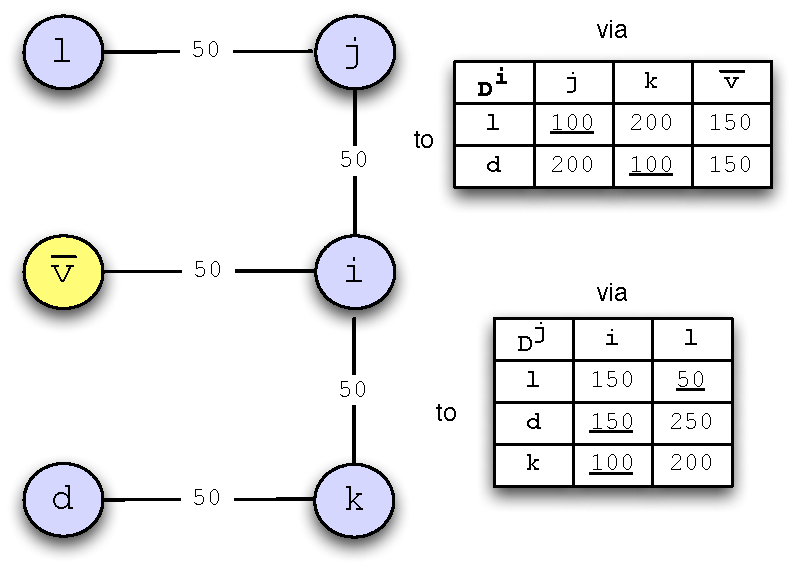
\includegraphics[scale=0.55]{figs/example-a-color.pdf}}
    \subfigure[After $\overline{v}$ is compromised. The dashed lines mark false paths claimed by $\overline{v}$.]
	{\label{fig:example-b}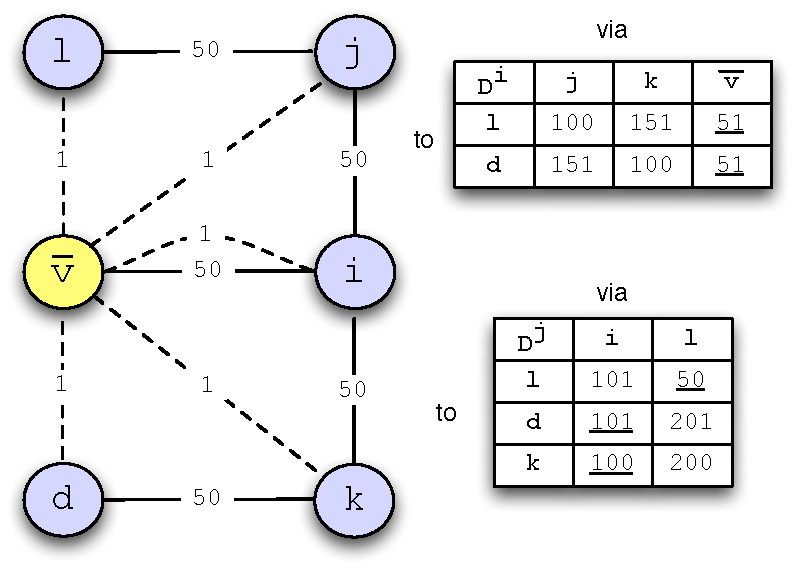
\includegraphics[scale=0.55]{figs/example-b-color.pdf}} 
    \subfigure[After recovery.]{\label{fig:example-c}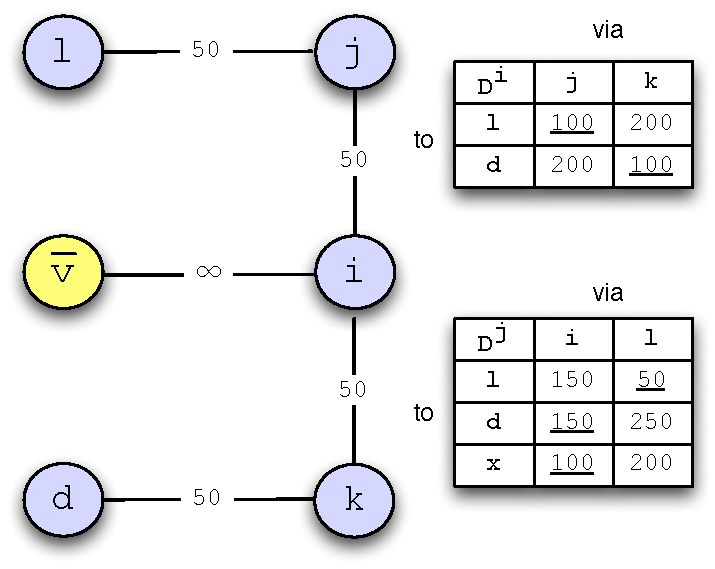
\includegraphics[scale=0.55]{figs/example-c-color.pdf}}
  \end{center}
	%\caption{Three snapshots of a graph, $G$.}
	\caption{Three snapshots of a graph, $G$, where $\overline{v}$ is the compromised node. Parts of $i$ and $j$'s distance matrix are displayed to the right of each sub-figure.
	The least cost values are underlined.}
	%$dmatrix_i$ and $dmatrix_j$ are displayed to the right of each sub-figure.
	%The least cost values are underlined.}
	%(a) $G$  before $\overline{v}$ is compromised, (b) $G$ after $\overrightarrow{bad}$ has}
	%has finished propagating but before recovery has started, and (c) $G$ after recovery. The dashed lines in (b) mark false paths used by $\overrightarrow{bad}$. 
	%Parts of $dmatrix_i$ and $dmatrix_j$ are displayed to the right of each sub-figure. The least cost values are underlined.}
  \label{fig:dv-example}
\end{figure*}


We trace the execution of \second using the example in Figure \ref{fig:dv-example}.
In Figure \ref{fig:example-b}, $i$ uses \bad to reach nodes $l$ and $d$.  $j$ uses $i$ to reach all nodes except $l$.  Notice that when $j$ uses $i$ to reach $d$, 
it transitively uses \badvector (e.g., uses path $j-i-$\bads$-d$ to $d$). 
After the preprocessing completes, $i$ selects a new neighbor to route through to reach $l$ and $d$ by finding its new smallest distance in \dmatrixi 
to these destinations: $i$ selects the routes via $j$ to $l$ with a cost of $100$ and $i$ picks the route via $k$ to reach $d$ with cost of $100$. 
(No changes are required to route to $j$ and $k$ because $i$ uses its direct link to these two nodes). 
Then, using traditional distance vector $i$ sends \minvi to $j$ and $k$.  When $j$ receives \minvis, $j$ must modify its distance to $d$ because \minvi indicates 
that $i$'s least cost to $d$ is now $100$.
$j$'s new distance value to $d$ becomes $150$, using the path $j-i-k-l$. $j$ then sends a message sharing \minvj with its neighbors.  From this point, recovery proceeds according 
by using traditional distance vector. 

%{\bf Pros/Cons.} 
\second is simple and makes no synchronization assumptions. % The primary advantage of \second is its simplicity.
However, \second is vulnerable to the \infinity problem. Because each node only has local information, the new shortest paths may continue to use \bads.
%When computing new shortest paths, a node cannot guarantee that the new shortest path does not use \bad because the node only has local information. 
For example, if $w(k,d)=400$ in Figure \ref{fig:dv-example}, a \infinity scenario would arise. After notification of \bads's compromise, 
$i$ would select the route via $j$ to reach $d$ with cost $151$ (by consulting \dmatrixis), using a path that does not actually exist in $G$ ($i-j-i-$\bads$-d$), since $j$ has removed \bad as a 
neighbor. When $i$ sends \minvi to $j$, $j$ selects the route via $i$
to $d$ with cost $201$. Again, the path $j-i-j-i-$\bads$-d$ does not exist.  In the next iteration, $i$ 
picks the route via $j$ having a cost of $251$. This process continues until each node finds their 
correct least cost to $d$.  We will see in our simulation study that the \infinity problem can incur significant message and time costs.




\subsection{The Purge Algorithm}
\label{subsec:purge}


\purge globally invalidates all false state using a diffusing computation and then uses distance vector to compute new distance values that avoid all invalidated paths.
Recall that diffusing computations preserve the decentralized nature of distance vector.
The diffusing computation is initiated at the neighbors of \bad because only these nodes are 
aware if \bad is used an intermediary node. The diffusing computations spread from \bads's neighbors to the network edge, invalidating false state at each node along the way. 
Then ACKs travel back from the network edge to the neighbors of \bads, indicating that the diffusing computation is complete. 
See Algorithm \ref{alg:purge} and \ref{alg:purge2} in the Appendix for a complete specification of this diffusing computation.

Next, \purge uses distance vector to recompute least cost paths invalidated by the diffusing computations.  In order to initiate the distance vector computation, each 
node is required to send a message after diffusing computations complete, even if no new least cost is found.  Without this step, distance vector may not correctly compute new least cost 
paths invalidated by the diffusing computations.  For example, consider the following the scenario when the diffusing computations complete: a node $i$ and all of $i$'s neighbors have 
least cost of $\infty$ to destination node $a$. Without forcing $i$ and its neighbors to send a message after the diffusing computations complete, neither $i$ nor $i$'s neighbors may
never update their least cost to $a$ because they may never receive a non-$\infty$ cost to $a$.

%{\footnote {\small The operations performed by the diffusing compuations described in Section \ref{subsec:preprocess} are  }
%This algorithm is specified in Algorithm \ref{alg:discover} of the Appendix.

In Figure \ref{fig:dv-example}, the diffusing computation executes as follows. First, $i$ sets its distance to $l$ and $d$ to $\infty$ (thereby invalidating $i$'s path to $l$ and $d$)
because $i$ uses \bad to route these nodes. Then, $i$ sends a message to $j$ and $k$ containing $l$ and $d$ as invalidated destinations.
When $j$ receives $i$'s message, $j$ checks if it routes via $i$ to reach $l$ or $d$. Because $j$ uses $i$ to reach $d$, $j$ sets its distance estimate to $d$ to $\infty$. 
$j$ does not modify its least cost to $l$ because $j$ does not route via $i$ to reach $l$. Next, $j$ sends a message that includes $d$ as an invalidated destination.
$l$ performs the same steps as $j$. After this point, the diffusing computation ACKs travel back towards $i$. When $i$ receives an ACK, the diffusing computation is complete. At this
point, $i$ needs to compute new least costs to node $l$ and $d$ because $i$'s distance estimates to these destinations are $\infty$. 
$i$ uses \dmatrixi to select its new route to $l$ (which is via $j$) and uses \dmatrixi to find $i$'s new route to $d$ (which is via $k$). Both new paths have cost $100$. Finally,
$i$ sends \minvi to its neighbors, triggering the execution of distance vector to recompute the remaining distance vectors.

Note that a consequence of the diffusing computation is that not only is all \badvector state deleted, but all \oldvector state as well.  
Consider the case when \bad is detected before node $i$ receives \badvectors.
It is possible that $i$ uses \oldvector to reach a destination, $d$. In this case, the diffusing computation will set $i$'s distance to $d$ to $\infty$.

An advantage of \purge is that it operates without the need for any clock synchronization.  We will find that \cprs, unlike \purges, either requires extra computation to maintain logical clocks or
assumes clocks are loosely synchronized. %no effort is required to synchronize clocks makes no synchronization assumptions. 
Also, \purges's diffusing computations ensure that the \infinity problem does not occur by removing
false state from the entire network. However, globally invalidating false state can be wasteful if valid alternate paths are locally available. 


\subsection{The CPR Algorithm}
\label{subsec:cpr}

\cprs {\footnote {\small The name is an abbreviation for {\bf C}heck{\bf P}oint and {\bf R}ollback. }} 
is our third and final recovery algorithm. 
Unlike \second and \purges, \cpr only requires that clocks across different
nodes be loosely synchronized i.e. the maximum clock offset between
any two nodes is assumed to be  bounded. For ease of explanation, we
describe \cpr as if the clocks at different nodes are perfectly
synchronized. Extensions to handle loosely synchronized clocks should
be clear. Accordingly, we assume that all neighbors of \bads, are
notified of the time, $t'$, at which \bad was compromised.  At the end of this section we comment on how the clock synchronization requirement assumption can be dropped by
using logical clocks.

For each node, $i \in G$, \cpr adds a time dimension to \minvi and \dmatrixis, which \cpr then uses to locally archive a complete history of values. 
Once the compromised node is discovered, 
the archive allows the system to rollback to 
a system snapshot from a time before \bad was compromised. From this point, \cpr needs to remove \bad and \oldvector and update stale distance values resulting from link weight changes.
We describe each algorithm step in detail. % (1) Create a \minv and \dmatrix archive. (2) roll back to a valid snapshot, and (3) steps after the rollback. 

{\bf Step 1: Create a \minv and \dmatrix archive.} 
	We define a  \emph{snapshot} of a data structure to be a copy of all current distance values along with a timestamp.
	{\footnote {\small In practice, we only archive distance values that have changed. Thus each distance value is associated with its own timestamp.}}
	The timestamp marks the time at which that set of distance values start being used. 
	\minv and \dmatrix are the only data structures that need to be archived. This approach is similar to ones used in temporal databases 
  \cite{Jensen91,Lomet06}.

  Our distributed archive algorithm is quite simple.  %For a given data structure, a node archives all current distance values whenever one of the values change. 
	Each node has a choice of archiving at a given frequency (e.g., every $m$ timesteps) or after some number of distance value changes (e.g., each time a distance 
	value changes).  Each node must choose the same option, which is specified as an input parameter to \cprs. A node archives independently of all other nodes.
  A side effect of independent archiving, is that even with perfectly synchronized clocks, the union of all snapshots may not constitute a globally consistent snapshot. 
  For example, a link weight change event may only have propagated 
  through part of the network, in which case the snapshot for some nodes will reflect this link weight change (i.e., among nodes that have learned of the event) 
  while for other nodes no local snapshot will reflect the occurrence of this event. We will see that a globally consistent snapshot is not required for correctness.  

{\bf Step 2: Rolling back to a valid snapshot.} 
Rollback is implemented using diffusing computations. Neighbors of the compromised node independently select a snapshot to roll back to, such that the snapshot is the most recent one taken
before $t'$.  Each such node, $i$, rolls back to this snapshot by restoring the \minvi and \dmatrixi values from the snapshot.  Then, $i$ initiates a diffusing computation to inform all other
nodes to do the same. If a node has already rolled back and receives an additional rollback message, it is ignored. 
(Note that this rollback algorithm ensures that no reinstated distance value uses \badvector because every node rolls back to a snapshot 
with a timestamp less that $t'$).  A pseudo-code specification of this rollback algorithm can be found in the Appendix (Algorithm \ref{alg:rollback}).  
%in the Appendix gives the pseudo-code for the rollback algorithm.


{\bf Step 3: Steps after rollback.} After Step 2 completes, the algorithm in Section \ref{subsec:preprocess} is executed.
There are two issues to address.
First, some nodes may be using \oldvectors.  Second, some nodes may have stale state as a result of link weight changes that occurred during $[t',t_b]$ and 
consequently are not reflected in the snapshot. 
To resolve these issues, each neighbor, $i$, of \bads, sets its distance to \bad to $\infty$ and then selects new least cost values that avoid the compromised node, triggering
the execution of distance vector to update the remaining distance vectors.  That is, for any destination, $d$, where $i$ routes via \bad to reach $d$,
$i$ uses \dmatrixi to find a new least cost to $d$. If a new least costs value is used, $i$ sends a distance vector message to its neighbors. Otherwise, $i$ sends no message.
Messages sent trigger the execution of distance vector.

During the execution of distance vector, each node uses the most recent link weights of its adjacent links. Thus, 
if the same link changes cost multiple times during  $[t',t_b]$, we ignore all changes but the most recent one. Algorithm \ref{alg:cpr} specifies Step 3 of \cprs.

In the example from Figure \ref{fig:dv-example}, the global state after rolling back is nearly the same as the snapshot depicted in Figure \ref{fig:example-c}:
the only difference between the actual system state and that depicted in Figure \ref{fig:example-c} is that in the former 
$(i,$\bads$)=50$ rather than $\infty$. Step 3 in \cpr makes this change.  Because no nodes use \oldvectors, no other changes take place.

Rather than using an iterative process to remove false state (like in \second and \purges), \cpr does so in one diffusing computation.
However, \cpr incurs storage overhead resulting from periodic snapshots of \minv and \dmatrixs.  Also, after rolling back, stale state may exist if link weight changes occur during $[t',t_b]$.
This can be expensive to update.
Finally, unlike \purge and \seconds, \cpr requires loosely synchronized clocks because without a bound on the clock offset, nodes may rollback to highly inconsistent local snapshots.
Although correct, this would severely degrade \cpr performance.

{\bf Using Logical Clock Timestamps.}
We can use Lamport's clock algorithm  \cite{Lamport78} to assign timestamps based on logical, rather than physical, clocks.  This allows us to drop the inconvenient assumption of loosely 
synchronized clocks. Here we briefly outline how the stated \cpr algorithm can be modified to use Lamport timestamps to create and restore system snapshots.

%First, \cpr is modified to create network-wide snapshots are periodically computed using diffusing computations instead of each node creating snapshots independently.   
First, \cpr is modified to create network-wide snapshots using diffusing computations instead of each node creating snapshots independently.   
Here each node records the logical timestamp when creating a checkpoint. 
The logical clock values are determined using the ``happened before'' relation defined by Lamport \cite{Lamport78}, where we limit events to be messages sent and received, and 
by piggybacking each node's logical clock value with each message it sends.  

%After being notified of \bads, each neighbor, $i$, of the compromised node determines the logical timestamp of the snapshot it wishes to restore.  
%This requires that either the detection algorithm specifies either \badvector or the logical time \bad was compromised. 
The second change to \cpr is in how each node determines the snapshot to restore during the roll back process (i.e., Step 2 above). Starting with each $i \in adj(\overline{v})$, 
$i$ determines the logical timestamp of the snapshot it wishes to restore.  This requires that the detection algorithm specifies either \badvector or the logical time \bad was compromised. 
In the latter case, finding the appropriate snapshot to restore is straightforward.
If only \badvector is provided, $i$ must additionally record each \minv vector received (as a part of standard distance vector messaging) 
along with the corresponding Lamport timestamp.  By doing so, this archive can be searched
to find the logical timestamp in which \badvector was first received at $i$.  Let $t_l$ denote this timestamp.  Next, $i$ initiates a diffusing computation instructing all other nodes 
to roll back to their most recent snapshot taken before $t_l$.  After this point, the diffusing computations continue as described in Step 2 above and Step 3 
remains unchanged.

Rolling back using logical timestamps does not guarantee that all \badvector state is removed because Lamport timestamps only provide partial ordering of events. 
With logical clocks, \cpr can be thought of as a best-effort approach to quickly removing false routing state by rolling back in time.  \cpr is still correct with logical clocks
for the reasons described in its correctness proof (Corollary \ref{cor:cpr-correct-single}).  
%This version of \cpr can be thought of as a best-effort approach to quickly removing false routing state.




\subsection{Multiple Compromised Nodes}
\label{subsec:mult}

Here we detail the necessary changes to each of our recovery algorithms when multiple nodes are compromised. Since we make the same changes to all three algorithms, we do not refer 
to a specific algorithm in this section. Let $\overline{V}$ refer to the set of nodes compromised at time $t'$. 

In the case where multiple nodes are simultaneously compromised, each recovery algorithm is modified such that for each $\overline{v} \in \overline{V}$, all $adj(\overline{v})$
are notified that \bad was compromised. 
%to accept a \emph{set} of compromised nodes, $\overline{V}$, as input (rather than a single node).  {\bf not really correct to refer to the set as input}
From this point, the changes to each algorithm are straightforward.  For example,
the diffusing computations described in Section  \ref{subsec:preprocess} are initiated at the neighbor nodes of each node in $\overline{V}$.
{\footnote {\small For \cprs, $t'$ is set to the time the first node is compromised.}}
%First, we augment the preceprocessing procedure described in Section \ref{subsec:preprocess}. In 
%the case where multiple nodes are simulataneously compromised, we modify the diffusing computations to remove all compromised nodes as a destination. %each of these nodes as a destination.

More changes are required to handle the case where an additional node is compromised during the execution of a recovery algorithm. Specifically, when another node is 
compromised, $\overline{v}_2$, we make the following change to the distance vector computation of each recovery algorithm.
{\footnote {\small {Recall that each of our recovery algorithms use distance vector to complete their computation.}} 
If a node, $i$, receives a distance vector message which includes a distance value to destination $\overline{v}_2$, then $i$ ignores said distance value and processes
the remaining distance values (if any exist) to all other destinations (e.g., where $d \neq \overline{v}_2$) normally.  If the message contains no distance information for any 
other destination $d \neq \overline{v}_2$, then $i$ ignores the message.
Because $\overline{v}_2$'s compromise 
triggers a diffusing computation to remove $\overline{v}_2$ as a destination, each node eventually learns the identity of $\overline{v}_2$, thereby allowing the node 
execute the specified changes to distance vector.

Without this change it is possible that the recovery algorithm will not terminate.  Consider the case of two compromised nodes, $\overline{v}_1$ and $\overline{v}_2$,
where $\overline{v}_2$ is compromised during the recovery triggered by $\overline{v}_1$'s compromise.  In this case, two executions of the recovery algorithm are triggered: one when
$\overline{v}_1$ is compromised and the other when $\overline{v}_2$ is compromised.
 Recall that all three recovery algorithms set all link weights to $\overline{v}_1$ to $\infty$ (e.g., $(v_i,\overline{v}_1)=\infty, \forall v_i \in adj(\overline{v}_1)$).
If the first distance vector execution triggered by $\overline{v}_1$'s compromise is not modified to terminate least cost computations to $\overline{v}_2$, the distance vector step of the 
recovery algorithm would never complete because the least cost to $\overline{v}_2$ is $\infty$. 






%%%%%%%%%%%%%%%% TRENDS IN RECOVERY SECTION %%%%%%%%%%
\section{Analysis of Algorithms}
\label{sec:analysis}

In Section \ref{subsec:correct}, we prove the correctness of our three
recovery algorithms.  Then, we prove specific properties of these
recovery algorithms in Section \ref{subsec:trends}, which help better
understand our simulation results.

\subsection{Correctness of Recovery Algorithms}
\label{subsec:correct}

%We first state our assumptions and then define correctness. Finally, we prove the correctness of each algorithm. 
We make the following assumptions in our proofs. All the initial \dmatrix values are nonnegative. Furthermore, all \minv values periodically
exchanged between neighboring nodes are nonnegative. 
All $v \in V$ know their adjacent link costs. All link weights in $G$ (and therefore $G'$ as well) are nonnegative and do not change.
{\footnote {\small We use the definition of $G$ and $G'$ described in Section \ref{sec:algs}.}}
$G$ is finite and connected. 

Finally, we assume reliable communication.


{\bf Definition 1.} An algorithm is \emph{correct} if the following two conditions are satisfied. One, $\forall v \in V$, $v$ has the least cost and knows next-hop to all destinations $v' \in V$.
Two, the least cost is computed in finite time.

%{\it Definition 2.} Let $D_i(t)$ be $i$'s least cost to node $d$ at time $t$, such that $d \neq i$. A distance value is \emph{incorrect} for node $i$ if $D_i(t') \neq D_i(t'')$ where 
%$t'$ is the current time and $t''$ marks the time the $D_i$ is first correct.

%{\it Definition 3.} An algorithm is \emph{recovery correct} if it is correct over $G'$.

{\bf Theorem 1}. {\it Distance vector is correct.}

$Proof$. Bertsekas and Gallager \cite{Gall87} prove correctness for distributed Bellman-Ford for arbitrary nonnegative \dmatrix values. 
Their distributed Bellman-Ford algorithm is the same as the distance vector algorithm used in this paper. \qed

{\bf Corollary 1}. {\it \second is correct.}

$Proof$. As per the preprocessing step, each node receiving a diffusing computation message removes \bad as a destination. 
Each node is guaranteed to receive a diffusing computation message (by our reliable communication and finite graph assumptions). Further, the diffusing computation
terminates in finite time.  Thus, we conclude that each $v \in V'$ removes \bad in finite time.

Following the diffusing computation, each $v \in adj($\bads$)$ uses distance vector to determine new least cost paths.
Because all \dmatrixv are nonnegative for all $v \in V'$, by Theorem $1$ we conclude \second is correct. \qed

{\bf Corollary 2}. {\it \purge is correct.}

$Proof$. The diffusing computation starts with each $v \in adj($\bads$)$ finding every destination, $d$, to which $v$'s least cost path 
uses \bad as the first-hop node. $v$ sets its least cost to each such $d$ to $\infty$, thereby invalidating its path to $d$.  
$v$ then initiates a diffusing computation. When an arbitrary node, $i$, receives a diffusing computation message from $j$, $i$ iterates 
through each $d$ specified in the message. If
$i$ routes via $j$ to reach $d$, $i$ sets its least cost to $d$ to $\infty$, therefore invalidating any path to $d$ with $j$ and  
\bad an intermediate nodes.  

By our assumptions, each node receives a diffusing computation message and the diffusing computation terminates in finite time. Thus, we conclude that all paths using \bad as an intermediary
node are invalidated in finite time. Following the preprocessing, each $v \in adj($\bads$)$ uses distance vector to determine new least cost paths.
Because all \dmatrixv are nonnegative for all $v \in V'$, by Theorem $1$ we conclude that \purge is correct. \qed

{\bf Corollary 3}. {\it \cpr is correct.}

$Proof$. \cpr rolls back using a diffusing computation. Each node that receives a diffusing computation message, rolls back to a snapshot with timestep less than $t'$.
By our assumptions, all nodes receive a message and the diffusing computation terminates in finite time.  Thus, we conclude
that each node $v \in V'$ rolls back to a snapshot with timestamp less than $t'$ in finite time.

\cpr then runs the preprocessing algorithm described in Section \ref{subsec:preprocess}, which removes \bad as a destination in finite time (as shown
in Corollary $1$). Because each node rolls back to a snapshot in which all least costs are nonnegative and 
\cpr then uses distance vector to compute new least costs, by Theorem $1$ we conclude that \cpr is correct. \qed

\subsection{Properties of Recovery Algorithms}
\label{subsec:trends}

In this section we formally characterize how \minv values change during recovery. The properties established in this section will aid
in understanding the simulation results presented in Section \ref{sec:eval}. Our proofs assume that link costs remain fixed during recovery (i.e., during $[t',t]$).
We prove properties about \minv in order provide a precise characterization of recovery trends.  
In particular, our proofs establish that:
%We do not characterize system behavior for \second
%and \cpr in this section becuase their behavior is relatively simple.  Instead, we wait until the evaluation section (Section \ref{sec:eval}) 
%to present their recovery trends. 

\begin{itemize}
	\item The least cost between two nodes at the start of recovery is less than or equal to the least cost when recovery has completed. (Theorem $2$)
	%That is, once the effects of the compromised node have been removed from the network, path costs cannot decrease. 

	\item Before recovery begins, if the least cost between two nodes is less than its cost when recovery is complete, the path must 
  be using \badvector or \oldvector either directly or transitively. (Corollary $4$)

	\item During \second and \cpr recovery, if the least cost between two nodes is less than its distance when recovery is complete, the path must 
  be using \badvector or \oldvector either directly or transitively. (Corollary $5$)

	%\item During recovery, if the least cost between two nodes exceeds the cost when recovery is complete then the node has yet to learn about the path used 
  	%when recovery is complete. (Claim $2$)

\end{itemize}

The first two statements apply to any recovery algorithm because they make no claims about \minv values during recovery. 
%These results are only relevant to \second and \purge recovery. \minv values during \cpr recovery do not follow these rules because it is possible
%that when rolling back link costs have different values such that the conditions for our claims below do not hold.

{\bf Notation}. We use the definition of $G$ and $G'$ described in Section \ref{sec:algs}. 
%$G=(V,E)$, with weight function $w: E \rightarrow \mathbb{N}$ and
%$G$ is undirected. $G'=(V',E')$, where $V' = V -$ \bad, $E'=E - \{(\bar{v},v_i)$ $|$ $v_i =adj(\bar{v}) \}$, edge weight function $w: E \rightarrow \mathbb{N}$, and $G'$ is undirected. 
Let $n,d \in V'$. Let $p_s(n,d)$ be the least cost path from node $n$ to $d$ at the start of recovery and $\delta_s(n,d)$ the
cost of this path; $p_i(n,d)$ is a path from $n$ to $d$ used during the recovery 
and $\delta_i(n,d)$ the cost of this path 
{\footnote {\small $p_i(n,d)$ and $\delta_i(n,d)$ can change over time during recovery.}}; and $p_f(n,d)$ the least cost path from $n$ to $d$ 
when recovery is finished and has cost $\delta_f(n,d)$.  %Using this notation we derive the following relationships. 
%Note by path we refer both to the nodes used to get from $n$ to $d$ and the cost of this path.  


{\bf Theorem 2.} $\forall n,d\in V'$, $ \delta_s(n,d) \leq \delta_f(n,d)$.

$Proof$: Assume $\exists n_i,d_i\in V'$ such that $\delta_s(n_i,d_i) > \delta_f(n_i,d_i)$.  The paths available at the start of recovery are a superset of 
those available when recovery is complete. This means $p_f(n_i,d_i)$ is available before recovery begins. Distance vector would use this path rather
than $p_s(n_i,d_i)$, implying that $\delta_s(n_i,d_i)=\delta_f(n_i,d_i)$, a contradiction. \qed

{\bf Corollary 4.} {\it $\forall n,d\in V'$, if $\delta_s(n,d) < \delta_f(n,d)$, then $p_s(n,d)$ is using \badvector or \oldvector either directly or transitively.}

$Proof$:  Assume $\exists n_i,d_i\in V$ such that a path $p_{s}(n_i,d_i)$ with cost $\delta_{s}(n_i,d_i)$ is used before recovery begins where
$\delta_{s}(n_i,d_i) < \delta_f(n_i,d_i)$ and  $p_{s}(n_i,d_i)$ does not use \badvector or \oldvectors.  The only paths available before recovery begins, which do not 
exist when recovery completes, are ones using \badvector or \oldvectors. Therefore, $p_{s}(n_i,d_i)$ must be available after recovery completes since we have assumed that
$p_{s}(n_i,d_i)$ does not use \badvector or \oldvector. Distance vector would use  $p_{s}(n_i,d_i)$ instead of $p_f(n_i,d_i)$ because 
$\delta_{s}(n_i,d_i) < \delta_f(n_i,d_i)$.  However this would 
imply that $\delta_{s}(n_i,d_i)= \delta_f(n_i,d_i)$, a contradiction. \qed

{\bf Corollary 5.} {\it For \second and \cprs. $\forall n,d\in V'$, if $\delta_i(n,d) < \delta_f(n,d)$ 
  then $p_i(n,d)$  must be using \badvector or \oldvector either directly or transitively} 
 {\footnote {\small Corollary 5 does not apply to \purge recovery because the  $\delta_i(n,d) < \delta_f(n,d)$ condition is not always satisfied.}} 

$Proof$: We can use the same proof for Corollary 4 if we substitute $\delta_i(n,d)$ for $\delta_s(n,d)$ and $p_i(n,d)$ for $p_s(n,d)$. \qed


%%%%%%%%%%%%%%%%%%%%% Begin COMMENT %%%%%%%%%%%%%%%%%%%%%%%%
\begin{comment}
Corollary 2 does not apply to \purge recovery because the  $\delta_i(n,d) < \delta_f(n,d)$ may not necessarily be satisfied. This is the case
because \infinity messages are not possible with \purge.

%Corollary 2 does not apply to \purge and \cpr recovery because the  $\delta_i(n,d) < \delta_f(n,d)$ may not necessarily be satisfied. Count-to-infinity
%messages are not possible with \purge so this condition is never met. With \cpr, it is possible that the state of a \minv used after rolling
%back does not satsify this condition because the \minv may reflect old link cost values that are less than their current values.
%These results establish that distance values before and during recovery are less than or equal to their final value. 
These results are useful in understanding recovery using \second and \cpr in cases where link costs remain fixed. With either algorithm,
our proofs imply that the general trend is for all \minv to increase from their value at the start of recovery up 
to their value when recovery has completed. Specifically, as a manifestation of the \infinity problem, paths using \badvector or \oldvector 
(with \cpr only \oldvector can be used as discussed in Section \ref{subsec:cpr}) are shared,
causing least cost paths to count up to their final value.  
There is one exception to this trend.  A node may learn of a new least 
cost path that uses \badvector or \oldvector with a cost less than any of its current least cost path, causing its least cost path to decrease. 

By Claim 1, \purge recovery also starts with \minv values less than or equal to their final value. However, for \purge \minv values actually 
count down from the $\infty$ costs set after the purge phase. 

%\cpr recovery trends are more difficult to characterize because link cost values can change between $t'$ and $t$.

We leverage these characterizations to explain our simulation results in the following section.
\end{comment}
%%%%%%%%%%%%%%%%%%%%% END COMMENT %%%%%%%%%%%%%%%%%%%%%%%%









\section{Evaluation}
\label{sec:eval}

In this section, we use simulations to characterize the performance of each of our three recovery algorithms in terms of message and time overhead. 
Our goal is to illustrate the relative performance of our recovery algorithms over different topology types (e.g., \er graphs, Internet-like graphs) and
different network conditions (e.g., fixed link costs, changing link costs).


%We build a custom simulator with a synchronous communication model: nodes send and receive messages at fixed epochs.  In each epoch, a node receives a
%message from all its neighbors and performs its local computation.  In
%the next epoch, the node sends a message (if needed).   All algorithms
We build a custom simulator with a synchronous communication model as described in Section \ref{sec:analysis}. All algorithms
are deterministic under this communication model.
The synchronous communication model, although simple, yields
interesting insights into the performance of each of the recovery
algorithms. Evaluation of our algorithms using a more general
asynchronous communication model is currently under
investigation. However, we believe an asynchronous implementation
will demonstrate similar trends.  

%Except in the case where multiple nodes are compromised, we simulate the following scenario:
We simulate the following scenario: 
{\footnote {\small In Section \ref{subsubsec:many} we consider the case of multiple compromised nodes.  In that experiment we modify our simulation scenario
to consider a set of compromised nodes, $\overline{V}$, instead of \bads.}}
\begin{enumerate}
	\item Before $t'$, $\forall v \in V$ \minvv and \dmatrixv are correctly computed.

	\item At time $t'$, \bad is compromised and advertises a \badvector (a vector with a cost of $1$ to \emph{every} node in the network) to its neighboring nodes.

	\item \badvector spreads for a specified number of hops (this varies by experiment).  Variable $k$ refers to the number of hops that \badvector has spread.

	\item At time $t$, some node $v \in V$ notifies all $v \in adj($\bads$)$ that \bad was compromised. 
	{\footnote { \small For \cpr this node also indicates the time, $t'$, \bad was compromised.}} 

\end{enumerate}
The message and time overhead are measured in step (4) above. The pre-computation common to all three recovery algorithms, described in Section \ref{subsec:preprocess},
is not counted towards message and time overhead. We describe our simulation scenario for multiple compromised nodes in Section \ref{subsubsec:many}.


\subsection{Fixed Link Weight Experiments}
\label{subsec:fixed}

In the next five experiments, we evaluate our recovery algorithms over different topology types in the case of fixed link costs.

\subsubsection{Experiment 1 - \er Graphs with Fixed Unit Link Weights}
\label{subsubsec:expt1}

We start with a simplified setting and consider 
Erd\"{o}s-R\'enyi graphs with parameters $n$ and $p$. 
$n$ is the number of graph nodes and $p$ is the probability that link $(i,j)$ exists where $i,j \in V$.
The link weight of each edge in the graph is set to $50$.
We iterate over different values of $k$. For each $k$, we 
generate an Erd\"{o}s-R\'enyi graph, $G = (V,E)$, with parameters $n$ and $p$. Then we select a \bad $\in V$ uniformly at random and simulate the scenario described above, 
using \bad as the compromised node. In total we sample $20$ unique nodes for each $G$.
We set $n=100$, $p=\{0.05,0.15,0.25, 0.50\}$, and let $k=\{1,2,
... 10\}$. Each data point is an average over $600$ runs ($20$ runs over 
$30$ topologies).  We then plot the $90 \%$ confidence interval.

For each of our recovery algorithms, Figure \ref{fig:msg} shows the
message overhead for different values of $k$. %The $90 \%$ confidence interval is shown.
We conclude that \cpr outperforms \purge and \second across all topologies. \cpr performs well because \badvector is removed using a single diffusing computation,  
while the other algorithms remove \badvector state through distance vector's iterative process.
\cprs's global state after rolling back is almost the same as the final recovered state.

\begin{figure*}[t]
\centering
\subfigure[{$p=0.05$, diameter=$6.14$}]{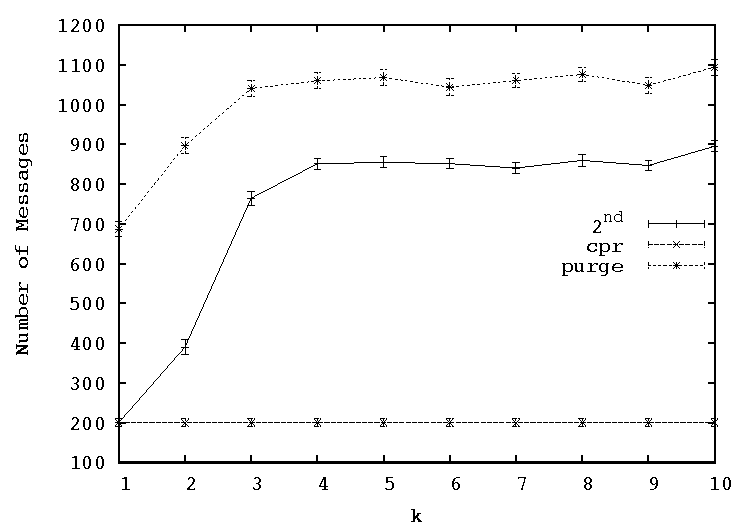
\includegraphics[width=0.32\textwidth]{figs/synch/msg5.pdf}}
\subfigure[{$p=0.15$, diameter=$3.01$}]{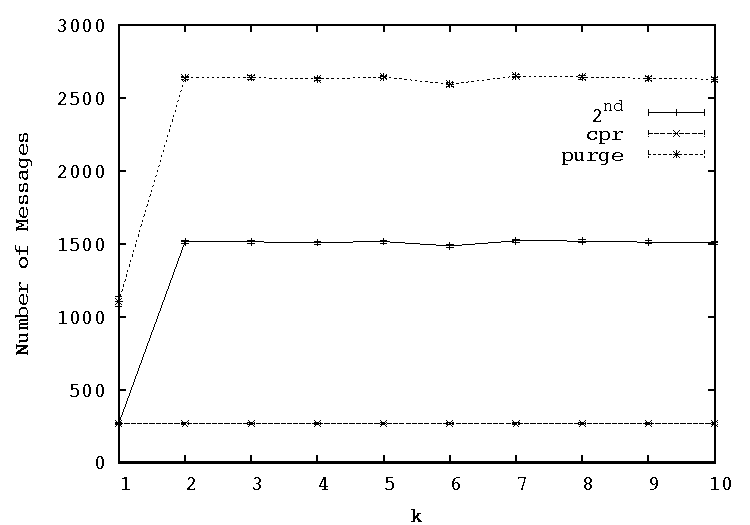
\includegraphics[width=0.32\textwidth]{figs/synch/msg15.pdf}}
\subfigure[{$p=0.25$, diameter=$2.99$}]{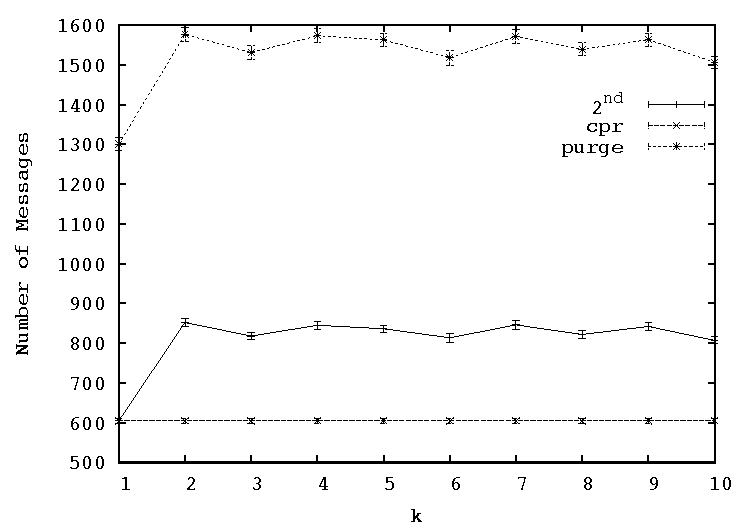
\includegraphics[width=0.32\textwidth]{figs/synch/msg25.pdf}}
\subfigure[{$p=0.50$, diameter=$2$}]{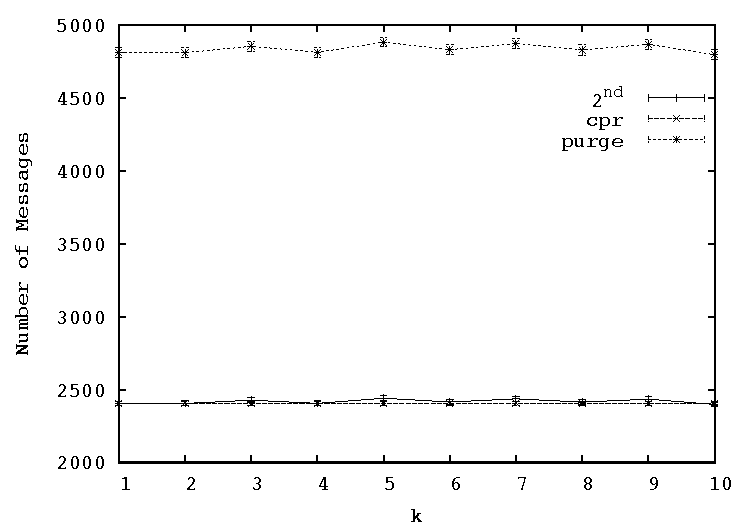
\includegraphics[width=0.32\textwidth]{figs/synch/msg50.pdf}}
%\subfigure[{Cumulative path cost decreases during the simulation}]{\includegraphics[width=0.49\textwidth]{figs/tsdecrease6.pdf}}
\caption{Experiment 1: message overhead for \er Graphs with Fixed Unit Link Weights generated over different $p$ values. Note the y-axis have different scales.}
\label{fig:msg}
\end{figure*}

\begin{figure*}[t]
\centering
\subfigure[{$p=0.05$, diameter=$6.14$}]{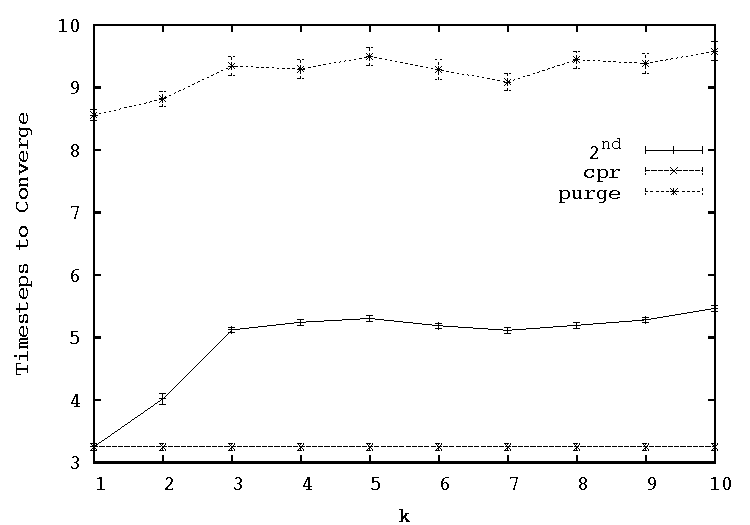
\includegraphics[width=0.32\textwidth]{figs/synch/epoch5.pdf}}
\subfigure[{$p=0.15$}, diameter=$3.01$]{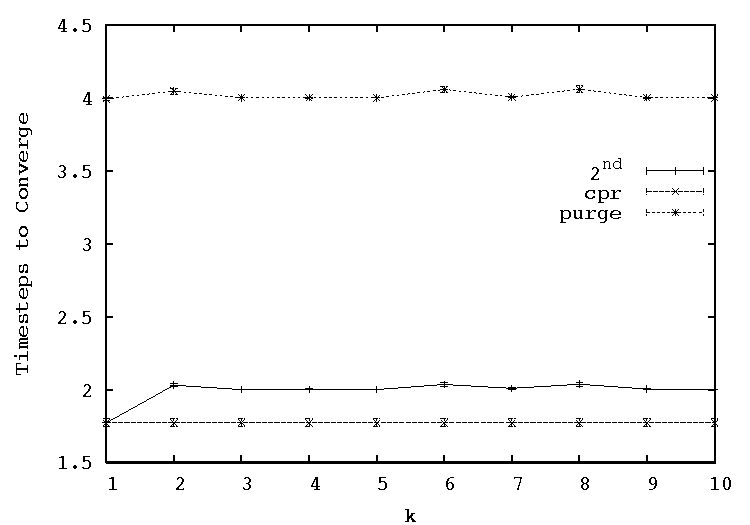
\includegraphics[width=0.32\textwidth]{figs/synch/epoch15.pdf}}
\subfigure[{$p=0.25$}, diameter=$2.99$]{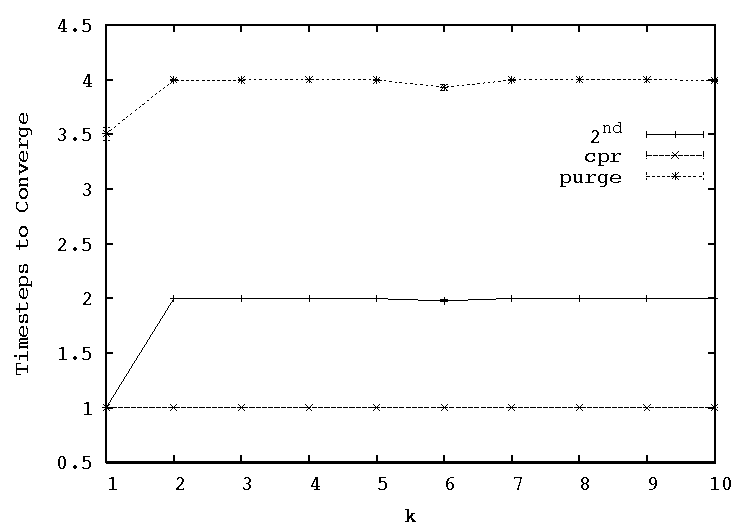
\includegraphics[width=0.32\textwidth]{figs/synch/epoch25.pdf}}
\subfigure[{$p=0.50$}, diameter=$2$]{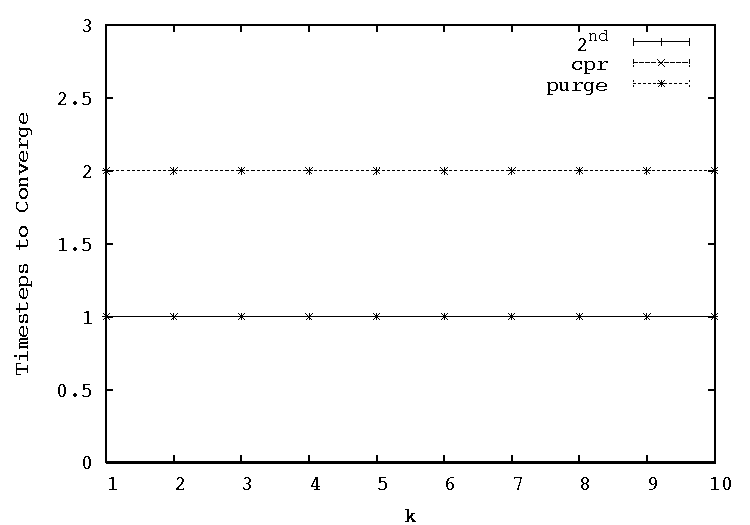
\includegraphics[width=0.32\textwidth]{figs/synch/epoch50.pdf}}
%\subfigure[{Cumulative path cost decreases during the simulation}]{\includegraphics[width=0.49\textwidth]{figs/tsdecrease6.pdf}}
\caption{Experiment 1: time overhead for \er Graphs with Fixed Unit Link Weights generated over different $p$ values.}
\label{fig:epoch}
\end{figure*} 


%In other words, \cpr performs well because its global state  (recall we define the global state of the routers as the union of their local states) is almost the same as the final recovered state.
%Specifically, if we let $S'$ represent the global state after rolling back and let $S$ be the final recovered state, the only difference between $S$ and $S'$, is that $S'$ 
%contains state that depends directly or transitively on \oldvector while $S$ does not. 
%\cpr performs exactly the same as \second at $k=1$ because \second at $k=1$ also must only remove \oldvector state and uses the same iterative process as \cprs. 
%For this reason, across all $k$ values, \cpr performs exactly the same as \second at $k=1$.  {\bf note:} {\it may need to elaborate more here.}

\second recovery can be understood as follows.  By Corollary \ref{cor:startbad} and \ref{cor:during} in Section \ref{subsec:trends}, distance values increase from their initial value until they 
reach their final (correct) value. Any intermediate, non-final, distance value uses \badvector or \oldvectors. Because \badvector and \oldvector no longer exist during recovery,
these intermediate values must correspond to routing loops.
%In this experiment, with \second distance estimates quickly count up to their final value.
Table \ref{tab:loop1} shows that there are few pairwise routing loops during \second recovery in the network scenarios generated in Experiment 1, 
indicating that \second distance values quickly count up to their final value.
{\footnote {\small We compute this metric as follows. After each simulation timestep, we count all pairwise routing loops over all source-destination pairs and then sum all of these values.}}
Although no pairwise routing loops exist during \purge recovery, \purge incurs overhead in performing network-wide state invalidation. Roughly, $50\%$ of \purges's messages come from these
diffusing computations. 
For these reasons, \purge has higher message overhead than \seconds.

Figure \ref{fig:epoch} shows the time overhead for the same $p$ values. The trends for time overhead match the trends we observe for message overhead. 
{\footnote {\small For the remaining experiments, we omit time overhead plots because time overhead follows the same trends as message overhead.}}


\begin{table}
\begin{center}
\begin{tabular}{l|l|l|l|l}
 & $k=1$&  $k=2$ & $k=3$ & $k=4-10$ \\
\hline
 $p=0.05$  & $0$ & $14$ & $87$ &  $92$ \\
 $p=0.15$  & $0$ & $7$&  $8$ & $9$ \\
 $p=0.25$  & $0$ & $0$ & $0$ &  $0$ \\
 $p=0.50$  & $0$ & $0$ & $0$ &  $0$ \\
 %$p=\{0.15,0.25,0.50\}$  & $0$ & $0$&  $0$ & $0$ \\
\end{tabular}
\end{center}
\caption{Average number pairwise routing loops for \second in Experiment 1.}
%$p=.50$ for Experiment 1 is omitted because no pairwise routing loops are found across all $k$ values.} 
\label{tab:loop1}
\end{table}

\begin{table}
\begin{center}
\begin{tabular}{l|l|l|l|l}
 & $k=1$&  $k=2$ & $k=3$ & $k=4-10$ \\
\hline
  $p=0.05$  & $554$ & $1303$ & $9239$ &  $12641$ \\
 $p=0.15$  & $319$ & $698$&  $5514$ & $7935$ \\
 $p=0.25$  & $280$ & $446$ & $3510$ &  $5440$ \\
 $p=0.50$  & $114$ & $234$ & $2063$ &  $2892$ \\
 %$p=\{0.15,0.25,0.50\}$  & $0$ & $0$&  $0$ & $0$ \\
\end{tabular}
\end{center}
\caption{Average number pairwise routing loops for \second in Experiment 2.}
%$p=.50$ for Experiment 1 is omitted because no pairwise routing loops are found across all $k$ values.} 
\label{tab:loop2}
\end{table}


\purge and \second message overhead increases with larger $k$. Larger $k$ imply that false state has propagated further in the network, 
implying more paths to repair, and therefore increased messaging.
For values of $k$ greater than a graph's diameter, the message overhead remains constant, as expected. 

%However, once $k$ is equal the graph diameter, $d$, the message overhead and number of epochs do not change for larger values of $k$ for a given topology. By definition, the graph diameter is
%the longest shortest path and so it follows that when $k > d$, each $v \in V'$ has a path less than $k$ hops to all destinations.  Therefore each $v$, does not use the $k$ hop path to \bads.
%For this reason, the message overhead (and number of epochs) do not change for $k>d$. {\bf todo verify if this is correct}

%Figure \ref{fig:compare} shows that for most values of $k$, if we do not count the epochs that occurred during \purges's purge phase 
%(e.g., only count \purges's discovery phase epochs), the resulting epoch omplexity is lower than \seconds's epoch complexity. When $k>2$, \second has higher epoch complexity 
%because the \infinity problem occurs with \second and not with \purges.  Table \ref{tab:loop1} shows that when $k>2$ there are pairwise routing loops during \second recovery, while

%The exception to this trend is when $k=1$ for all topologies and $k=2$ for $p=.05$: \purges's discovery phase epoch complexity is higher than \seconds's total epoch complexity. 
%In these cases, there are no or few pairwise routing loops for \seconds.  In this way, this is an ideal case for \second recovery. 
%Meanwhile, there are several cases in which distance values that previously used \oldvectors, which do not require messaging for \second but do for \purges.  
%Recall that \purge sets all distances that use \badvector or \oldvector to $\infty$ in its purge phase, so for \purge all distances using \oldvector must be recomputed. 
%With \seconds, many of these same distance values do not require re-computation: the actual path changes such as not to use \oldvector but the distance does not change because an 
%alternate path of the same distance is locally selected (since the distance does not change, no message is sent).


\subsubsection{Experiment 2 - \er Graphs with Fixed but Randomly Chosen Link Weights}
\label{subsec:expt2}


The experimental setup is identical to Experiment 1 with one exception: link weights are selected uniformly at random between $[1,n]$ (rather than using 
fixed link weight of $50$).

Figure \ref{fig:msg-rand} show the message overhead for different $k$ where $p=\{0.05,0.15,0.25,0.50 \}$. 
%We omit the figures for the other $p$ values because they follow the same trend as $p=.05$.
In striking contrast to Experiment 1, \purge outperforms \second for most values of $k$. 
\second performs poorly because the \infinity problem: Table \ref{tab:loop2} shows the large average number of pairwise routing loops in this experiment, 
an indicator of the occurrence of \infinity problem.
In the few cases (e.g., $k=1$ for $p=0.15$, $p=0.25$ and $p=0.50$) that \second performs better than \purges, \second has few routing loops.

No routing loops are found with \purges. \cpr performs well for the same reasons described in Section \ref{subsubsec:expt1}.  

\begin{figure*}[t]
\centering
\subfigure[{$p=0.05$, diameter=$6.14$}]{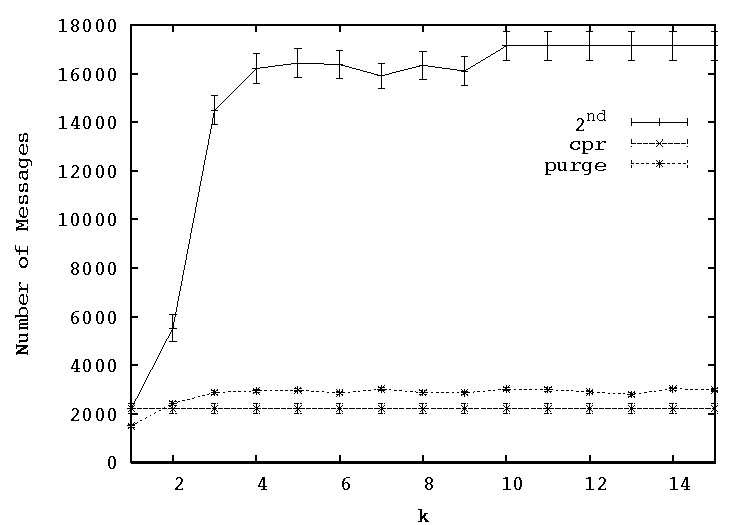
\includegraphics[width=0.32\textwidth]{figs/synch/msg-rand5.pdf}}
\subfigure[{$p=0.15$, diameter=$3.01$}]{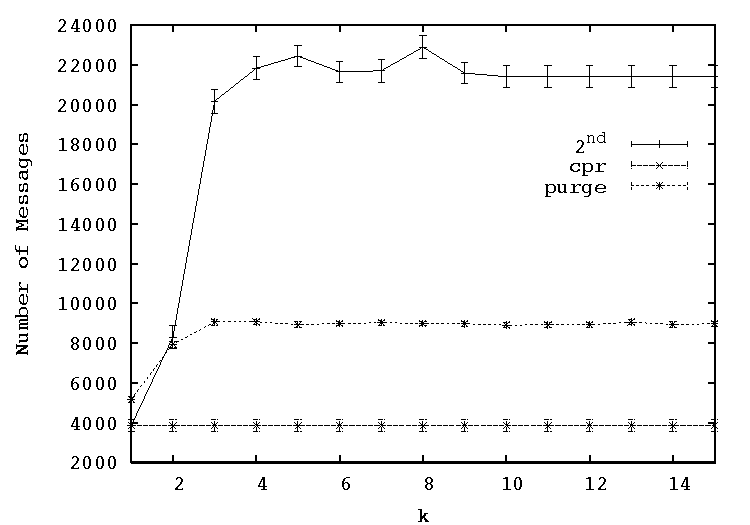
\includegraphics[width=0.32\textwidth]{figs/synch/msg-rand15.pdf}}
\subfigure[{$p=0.25$, diameter=$2.99$}]{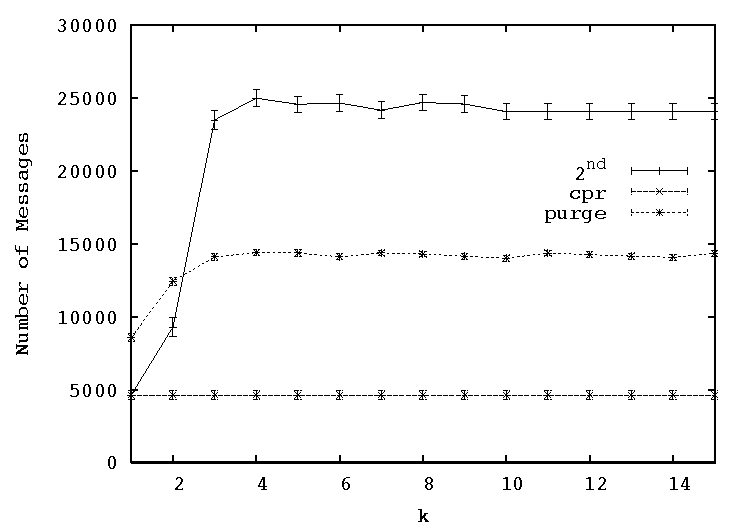
\includegraphics[width=0.32\textwidth]{figs/synch/msg-rand25.pdf}}
\subfigure[{$p=0.50$, diameter=$2$}]{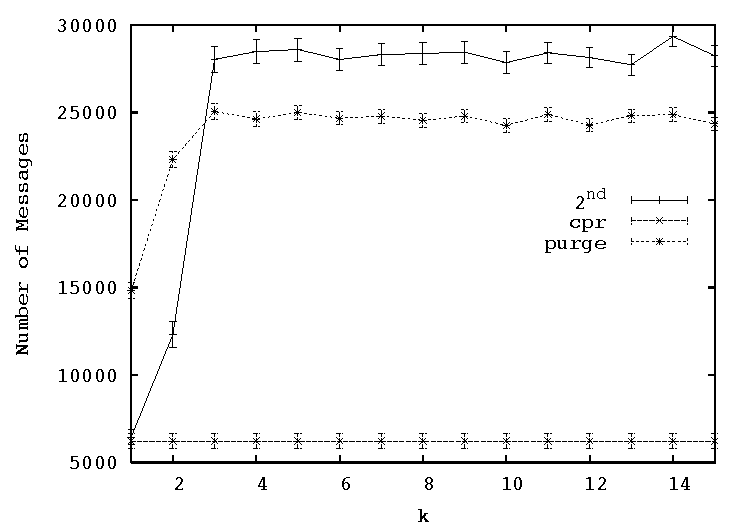
\includegraphics[width=0.32\textwidth]{figs/synch/msg-rand50.pdf}}
\caption{Experiment 2: message overhead for \er graph with link weights selected uniformly random from $[1,100]$. Note the y-axis have different scales.}
\label{fig:msg-rand}
\end{figure*}

%\begin{figure*}[t]
%\centering
%\subfigure[{$p=0.05$, diameter=$6.14$}]{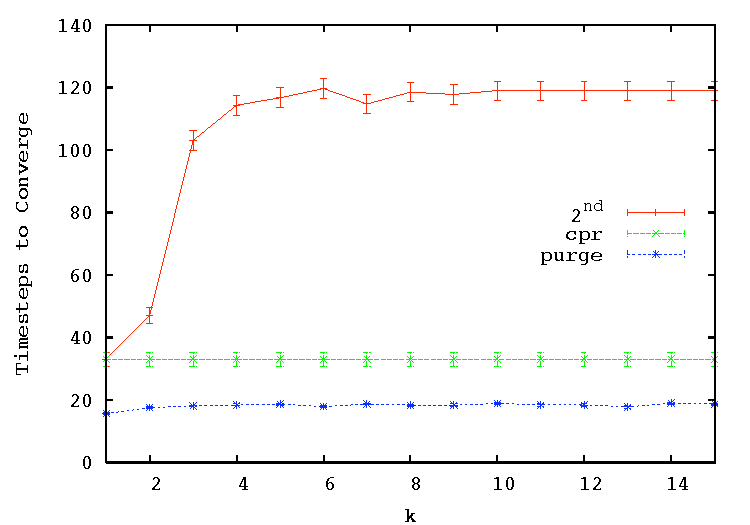
\includegraphics[width=0.32\textwidth]{figs/synch/epoch-rand5.pdf}}
%\subfigure[{$p=0.15$, diameter=$3.01$}]{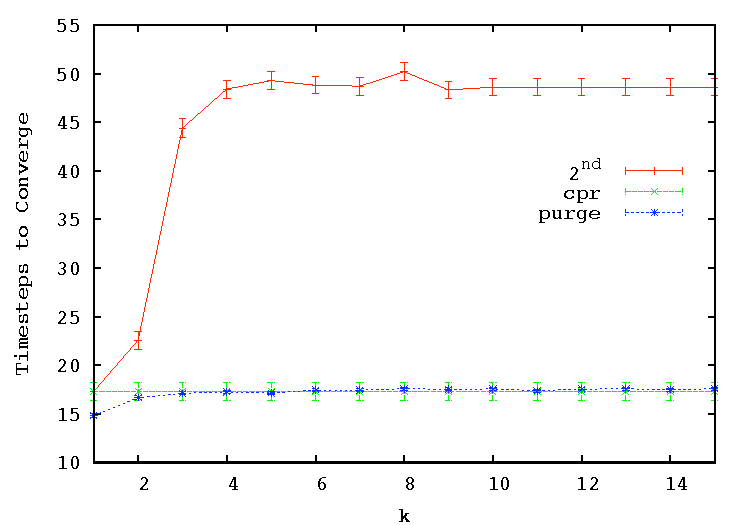
\includegraphics[width=0.32\textwidth]{figs/synch/epoch-rand15.pdf}}
%\subfigure[{$p=0.25$, diameter=$2.99$}]{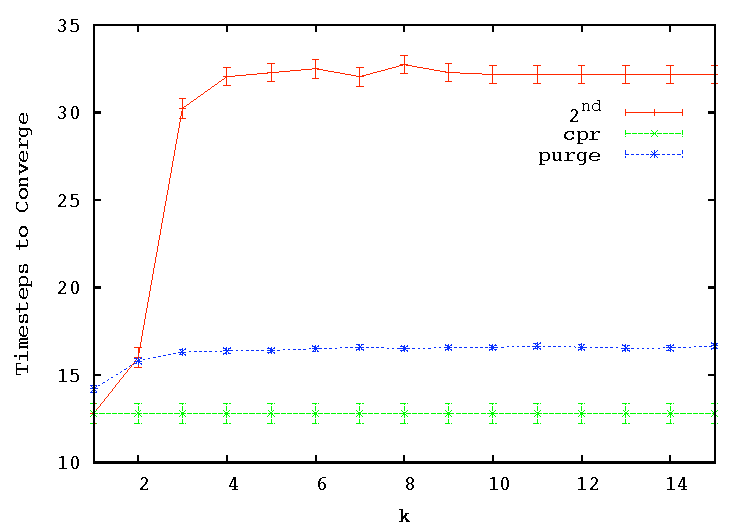
\includegraphics[width=0.32\textwidth]{figs/synch/epoch-rand25.pdf}}
%\subfigure[{$p=0.50$, diameter=$2$}]{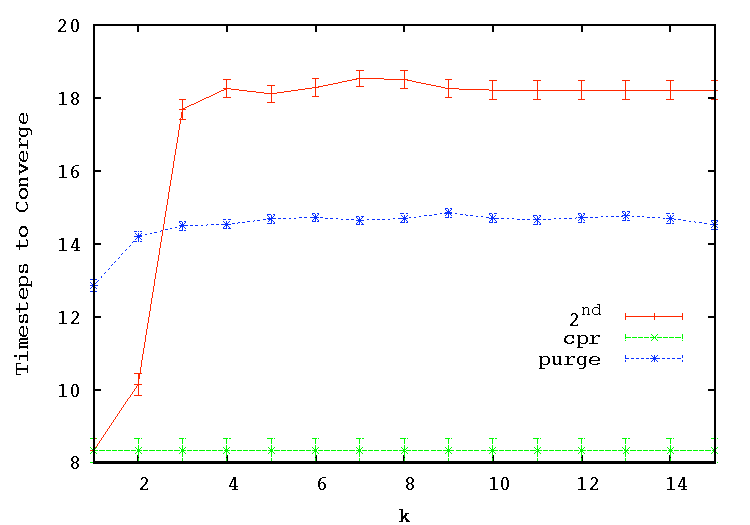
\includegraphics[width=0.32\textwidth]{figs/synch/epoch-rand50.pdf}}
%\subfigure[{Cumulative path cost decreases during the simulation}]{\includegraphics[width=0.49\textwidth]{figs/tsdecrease6.pdf}}
%\caption{Time overhead for \er graph with link weights selected uniformly random from $[1,100]$}
%\label{fig:epoch-rand}
%\end{figure*} 

%Recall that in Experiment 1, no pairwise routing loops are found when $p=0.15,p=0.25,$ and $p=0.50$.  The only pairwise routing loops in Experiment 1 
%are found when $p=0.05$, where a maximum of only $100$ pairwise routing loops occur. For \purges, no pairwise routing loops were found. {\bf Self-note}: {\it verify}.

In addition, we counted the number of epochs in which at least one pairwise routing loop existed.  For \second (across all topologies), on average, all but the last three 
timesteps had at least one routing loop.  This suggests that the \infinity problem dominates the cost for \seconds. 
%In some cases (e.g., $k=1$ for $p=.15$ and $p=.50$) \second performs better than \purges.  In these cases, \second has few routing loops.
%Table \ref{tab:loop} shows that there are fewer routing loops for small $k$. This is the case because with small $k$ there are fewer nodes using \badvectors. 

%The performance gap between \second and \purge shrinks with larger $p$ because with \second there are fewer routing loops with larger $p$.  
%This is consistent with our intuition:  larger $p$ values imply there are more alternate paths that do not use \badvectors.
%and thus routing loops are quickly exited because a low cost alternate path is used. 





\subsubsection{Experiment 3 - Internet-like Topologies}

%\begin{figure*}[t]
%\centering
%\subfigure[{AT\&T}]{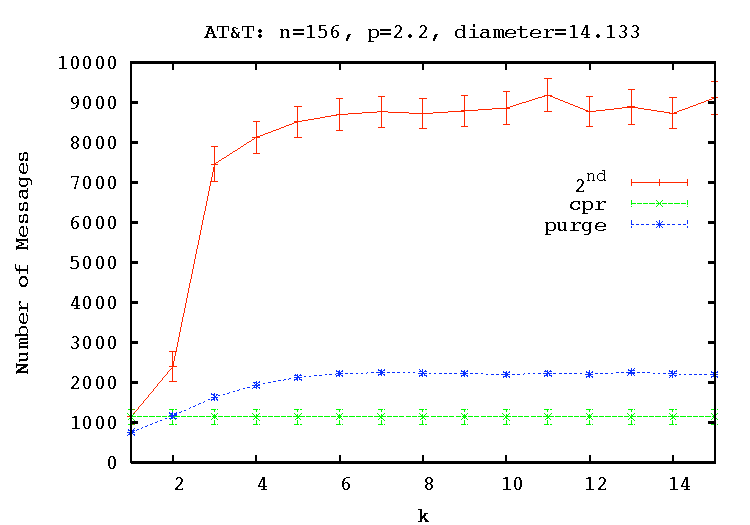
\includegraphics[width=0.32\textwidth]{figs/synch/att-msg.pdf}}
%\subfigure[{Rocketfuel 6461}]{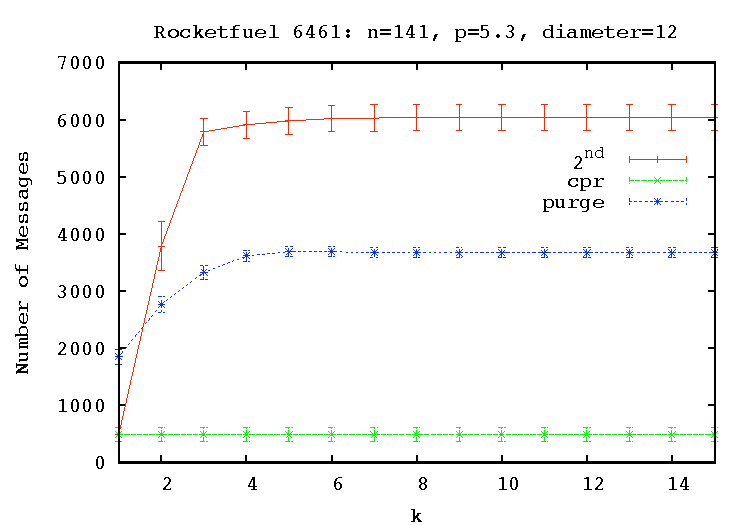
\includegraphics[width=0.32\textwidth]{figs/synch/rocket-msg6461.pdf}}
%\subfigure[{Rocketfuel 3867}]{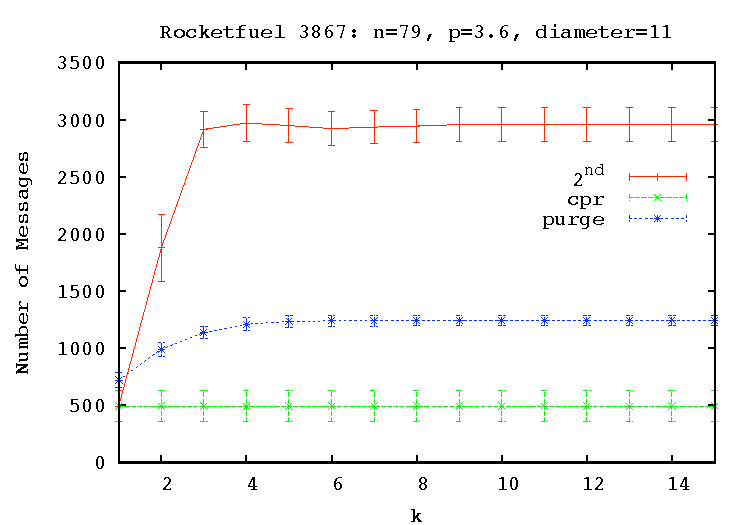
\includegraphics[width=0.32\textwidth]{figs/synch/rocket-msg3867.pdf}}
%\subfigure[{Cumulative path cost decreases during the simulation}]{\includegraphics[width=0.49\textwidth]{figs/tsdecrease6.pdf}}
%\caption{Real graph message overhead}
%\label{fig:msg-real}
%\end{figure*}


\begin{figure*}[t]
\centering
\subfigure[{GT-ITM, $n=156$, diameter=$14.133$}]{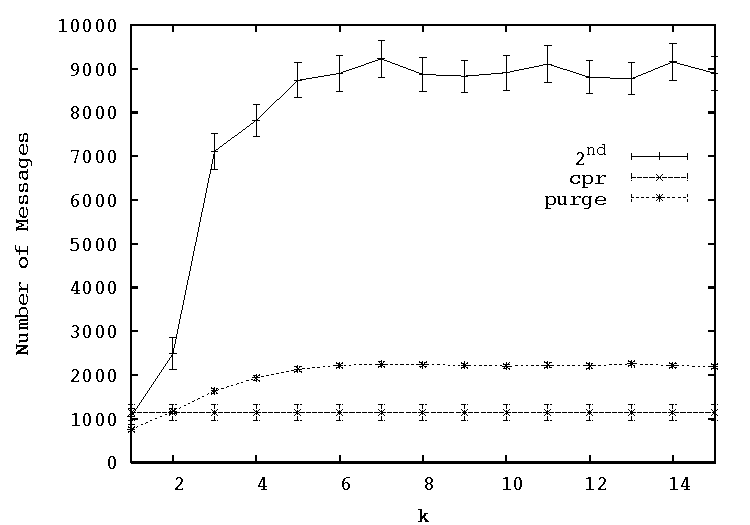
\includegraphics[width=0.32\textwidth]{figs/synch/msg-att.pdf}}
\subfigure[{Rocketfuel 6461, $n=141$, diameter=$8$}]{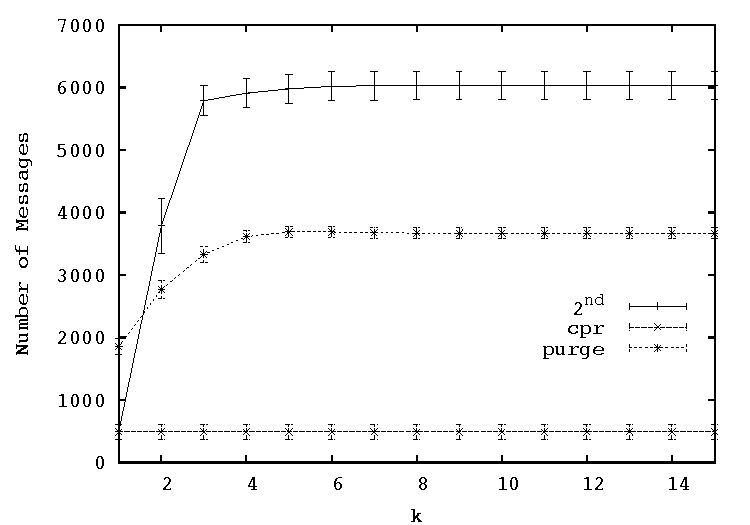
\includegraphics[width=0.32\textwidth]{figs/synch/msg6461.pdf}}
\subfigure[{Rocketfuel 3867, $n=79$, diameter=$10$}]{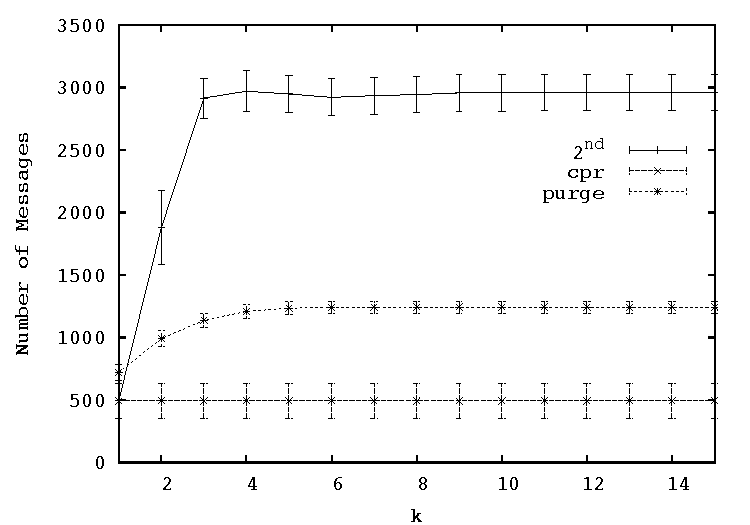
\includegraphics[width=0.32\textwidth]{figs/synch/msg3867.pdf}}
\caption{Experiment 3: Internet-like graph message overhead}
\label{fig:msg-real}
\end{figure*}

%\begin{figure*}[t]
%\centering
%\subfigure[{GT-ITM, $n=156$, average node degree=$2.2$, diameter=$14.133$}]{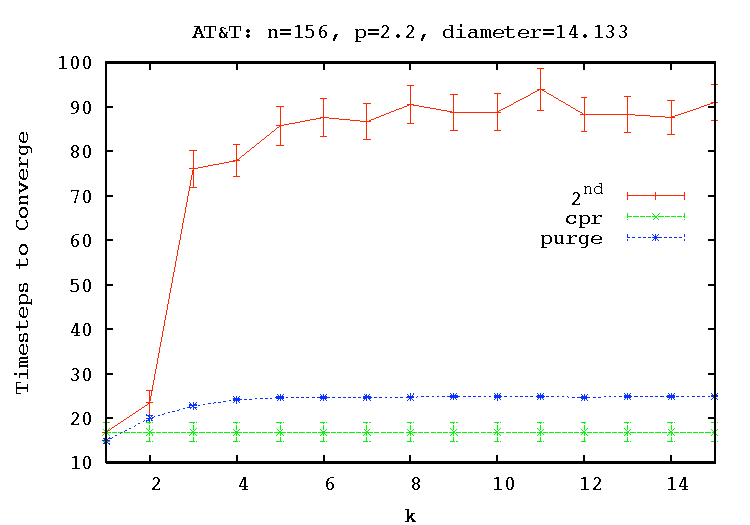
\includegraphics[width=0.32\textwidth]{figs/synch/att-epoch.pdf}}
%\subfigure[{Rocketfuel 6461, $n=141$, average node degree=$2.62$, diameter=$12$}]{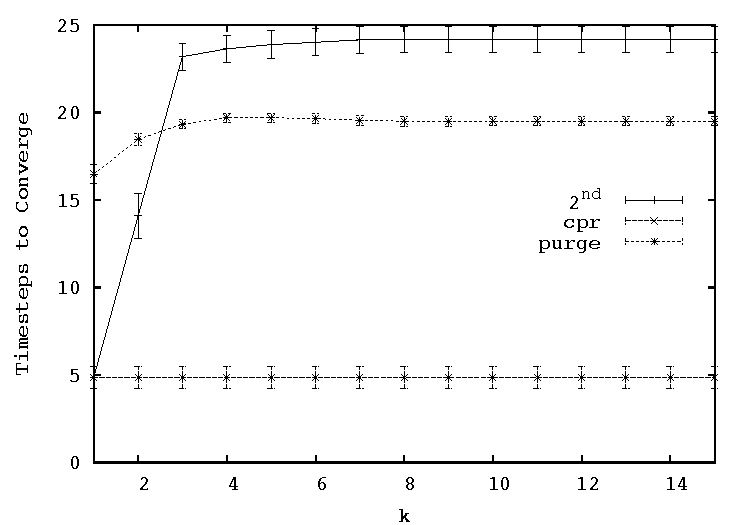
\includegraphics[width=0.32\textwidth]{figs/synch/rocket-epoch6461.pdf}}
%\subfigure[{Rocketfuel 3867, $n=79$, average node degree=$1.8$, diameter=$10$}]{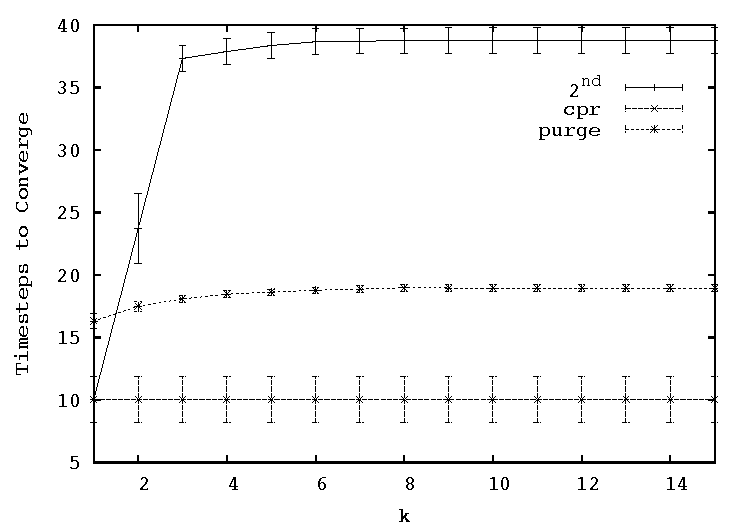
\includegraphics[width=0.32\textwidth]{figs/synch/rocket-epoch3867.pdf}}
%\subfigure[{Cumulative path cost decreases during the simulation}]{\includegraphics[width=0.49\textwidth]{figs/tsdecrease6.pdf}}
%\caption{Number of epochs/timesteps for real graphs}
%\label{fig:epoch-real}
%\end{figure*} 



Thus far, we studied the performance of our recovery algorithms over \er graphs, which have provided us with useful intuition about the performance
of each algorithm. In this experiment, we simulate our algorithms over Internet-like topologies downloaded from the Rocketfuel website \cite{Rocketfuel} and generated using GT-ITM 
\cite{GT-ITM}.  The Rocketfuel topologies have inferred edge weights. For each Rocketfuel topology, we let each node be
the compromised node and average over all of these cases for each value of $k$.  For GT-ITM, we used the parameters specified in Heckmann et al \cite{Heckmann} for  the $154$-node AT\&T topology
described in Section 4 of \cite{Heckmann}. For the GT-ITM topologies, we use the same criteria specified in Experiment 1 to generate each data point. 

The results, shown in Figure \ref{fig:msg-real}, follow the same pattern as in Experiment 2.  
%Due to space limitations, we only show the results for one representative topology.  The results for the other topologies follow the same pattern \cite{Tech}. 
In the cases where \second performs poorly,
the \infinity problem dominates the cost, as evidenced by the number of pairwise routing loops. In the few cases that \second performs better than \purges, there 
are few pairwise routing loops.

\subsubsection{Experiment 4 - Multiple Compromised Nodes}
\label{subsubsec:many}

In this experiment, we evaluate our recovery algorithms when multiple nodes are compromised. Our experimental setup is different from what we have used to this point:
we fix $k=\infty$ and vary the number of compromised nodes. Specifically, for each topology we create $m = \{1,2, ... , 15\}$ compromised nodes, each of which is selected  
uniformly at random (without replacement).  We then simulate the scenario described at the start of Section \ref{sec:eval} with one modification: $m$ nodes are 
compromised during $[t',t'+ 10]$. %We set $\Delta$ such that the recovery algorithm does not need to be restarted (as described in Section \ref{subsec:mult}).
The simulation is setup so that the outside algorithm identifies all $m$ compromised node at time $t$. %This eliminates the need to terminate and restart any recovery algorithm.
After running the simulation for all possible values for $m$, we generate a new topology and repeat the above procedure. 
We continue sampling topologies until the $90\%$ confidence interval for message overhead falls within $10\%$ of the mean message overhead. 

First, we perform this experiment using \er graphs with fixed link costs.  The message overhead results are shown in Figure \ref{fig:many-fixed}(a) for $p=0.05$ and $n=100$. 
{\footnote {\small We do not include the results for $p=\{0.15,0.25,0.50\}$ because they are consistent with the results for $p=0.05$.}}
The relative performance of the three algorithms is consistent with the results from Experiment 1, in which we had a single compromised node.
%We find the same trends we observed in Experiment 1 for large $k$ values in which there was a single compromised node.
As in Experiment 1, \second and \cpr have few pairwise routing loops (Figure \ref{fig:many-fixed}(b)).  In fact, there is more than an order of magnitude fewer pairwise routing 
loops in this experiment
when compared to the results for the same simulation scenario of $m$ compromised nodes using \er graphs with random link weights (Figure \ref{fig:many}(b)).
%The small number of pairwise routing loops is particularily evident when contrasted with the large number of pairwise routing loops 
%found with \er graphs with random link weights (Figure \ref{fig:many}(b)).  
Few routing loops imply that \second and \cpr (after rolling back) quickly count up to correct least costs.
In contrast, \purge has high message overhead because \purge globally invalidates false state before computing new least cost paths, rather than directly using alternate paths that 
are immediately available when recovery begins at time $t$. 
%The diffusing compuations are unnecessary in this scenario because many new least cost paths can be computed using local state information (demonstrated by \seconds's performance).

\second and \purge message overhead are nearly constant for $m \geq 8$ because at that point \badvector state has saturated $G$.
Figure \ref{fig:many-fixed} shows the number of least cost paths, per node,
that use \badvector or \oldvector at time $t$ (e.g., after \badvector state has propagated $k$ hops from \bads).  The number of least cost paths that use \badvector is nearly constant for $m \geq 8$. 

In contrast, \cpr message overhead increases with the number of compromised nodes.  After rolling back, \cpr must remove all compromised nodes and all
stale state (e.g., \oldvectors) associated with each \bads. As seen in Figure \ref{fig:many-fixed}(c), 
the amount of \oldvector state increases as the number of compromised nodes increase. 

Next, we perform the same experiment using \er graphs with with link weights selected uniformly at random from $[1,100]$. We only show the results for $p=.05$ and $n=100$ because the 
trends are consistent for other values of $p$.
The message overhead results for this experiment are shown in Figure \ref{fig:many}(a). \purge performs best because, unlike \second and \cprs, \purge does not suffer 
from the \infinity problem.  Below, we explain the performance of each algorithm in detail.

Consistent with Experiment 2 and 3, \second performs poorly because of the \infinity problem. 
Figure \ref{fig:many}(b) shows that a significant number of pairwise routing loops occur during \second recovery.  
\second message overhead remains constant when $m \geq 6$ because at this point \badvector state has saturated the network.  
Figure \ref{fig:many}(c) confirms this: the number of effected least cost paths remains constant (at $80$) for 
all $m \geq 6$. 

%\cpr also has a significant number of pairwise routing because after rolling back \cpr uses
%standard distance vector to compute new least cost paths for all paths using stale \oldvector state. Figure \ref{fig:many}(b) shows that the amount of \oldvector state increases as the
%number of compromised nodes increase, resulting in more routing loops for \cprs.

\cpr message overhead increases with the number of compromised nodes because the amount of \oldvector state increases as the number of compromised nodes increase (Figure \ref{fig:many}(c)). 
More \oldvector state results in more routing loops -- as shown in Figure \ref{fig:many}(b) -- causing increased message overhead.

%As with previous experiments,
\purge performs well because unlike \cpr and \seconds, no routing loops occur during recovery. %Figure \ref{fig:many}(b) shows that many pairwise routing loops occur during \second and \cpr recovery. 
Surprisingly, \purges's message overhead decreases when $m \geq 5$.  Although more 
least cost paths need to be computed with larger $m$, the message overhead decreases because the residual graph, $G'$, -- resulting from the removal of all $m$ compromised nodes -- is 
smaller than $G$.  As a result, there are $m$ fewer destinations and $m$ fewer nodes sending messages during the recovery process.
%As seen in Figure \ref{fig:many}(b), pairwise routing loops are prominent with both \second and \cprs. 

%used same topology for Rocketfuel ...
Finally, we simulated the same scenario of $m$ compromised node using the Internet-like graphs from Experiment 3. 
%{\footnote {\small For each Rocketfuel topology, we repeatidly selected $m$ compromised nodes until }}
The results were consistent with those for \er graphs with random link weights. % and therefore we do not present results for Internet-like graphs with multiple compromised nodes.



%Figure \ref{fig:many}(b) shows that the number of pairwise routing loops increases as the number of compromised nodes increases.  When $m \geq 6$, 
%in additional message overhead because more routing loops are processed per message. 
%{\bf think i want to remove the section about infinity message plot and the explanation about the number of loops per message}

\begin{figure*}[t]
\centering
\subfigure[{Message Overhead}]{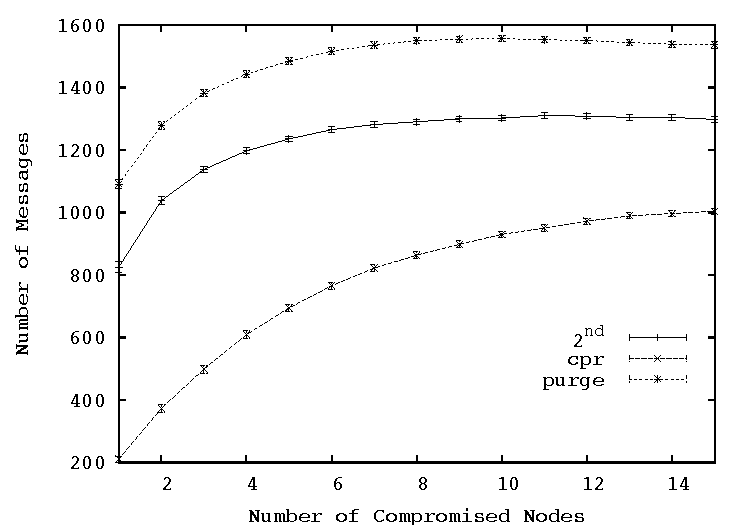
\includegraphics[width=0.32\textwidth]{figs/synch/many-fixed.pdf}}
\subfigure[{Pairwise Routing Loops}]{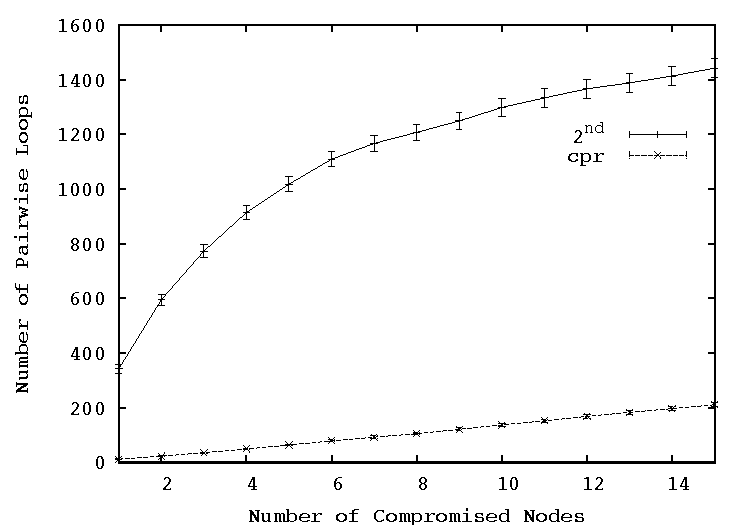
\includegraphics[width=0.32\textwidth]{figs/synch/loops-fixed.pdf}}
\subfigure[{Number of Effected Least Cost Paths}]{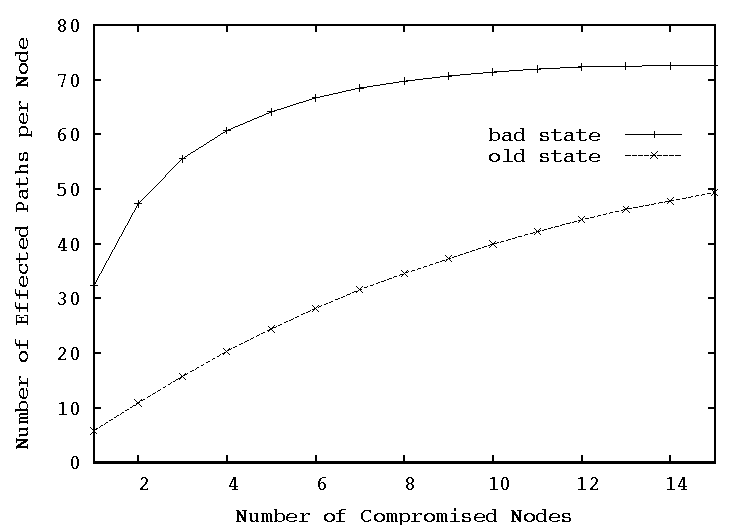
\includegraphics[width=0.32\textwidth]{figs/synch/initial-fixed.pdf}}
\caption{Experiment 4 - multiple compromised nodes over \er graphs with fixed link weights, $p=.05$, $n=100$, and diameter=$6.14$.}
\label{fig:many-fixed}
\end{figure*}



\begin{figure*}[t]
\centering
\subfigure[{Message Overhead}]{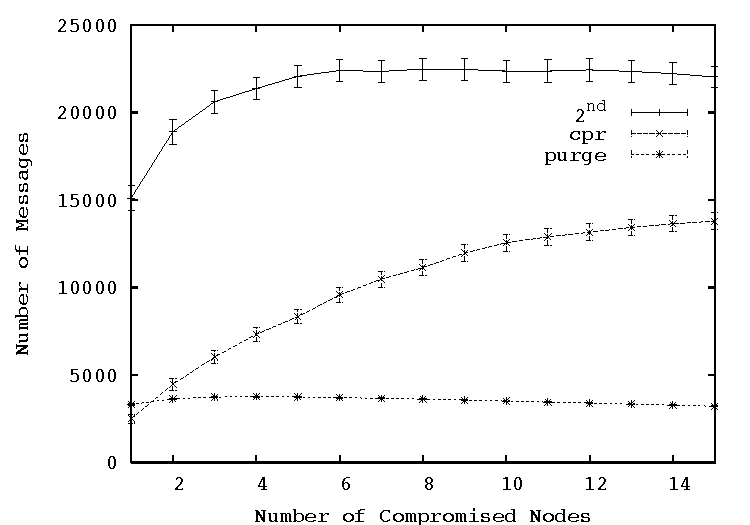
\includegraphics[width=0.32\textwidth]{figs/synch/many-rand.pdf}}
\subfigure[{Pairwise Routing Loops}]{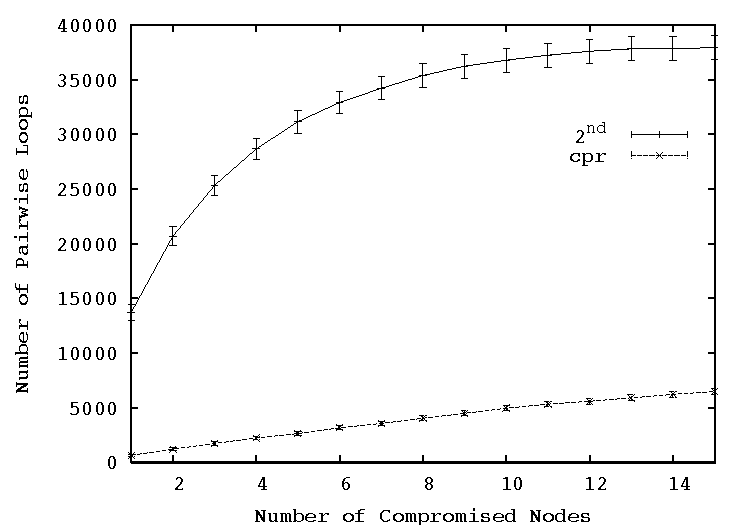
\includegraphics[width=0.32\textwidth]{figs/synch/loops-rand.pdf}}
\subfigure[{Number of Effected Least Cost Paths}]{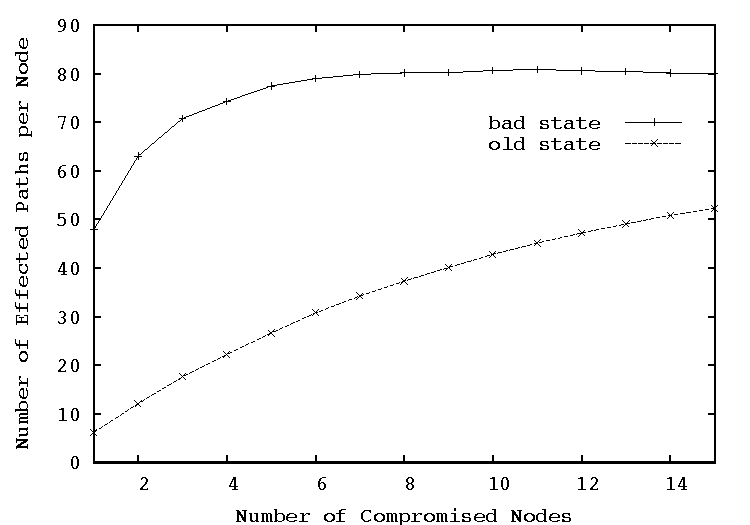
\includegraphics[width=0.32\textwidth]{figs/synch/initial-rand.pdf}}
\caption{Experiment 4 - multiple compromised nodes over \er graphs with link weights selected uniformly at random from $[1,100]$, $p=.05$, $n=100$, and diameter=$6.14$.}
\label{fig:many}
\end{figure*}

\subsubsection{Experiment 5 - Poison Reverse}
%Here we study the benefits of using poison reverse to \second and \cprs. 
We repeat Experiments 2, 3, and 4 using poison reverse for \second and \cprs.  
We do not apply poison reverse to \purge because no routing loops (resulting from the removal of \bads)
exist during \purges's recovery. Additionally, we do not repeat Experiment 1 using poison reverse because we observed few routing loops in that experiment. 

First, we repeat Experiment 2 using poison reverse. The results are shown for one representative topology in Figure \ref{fig:pr-fix}(a),
where \second + {\tt pr} and \cpr + {\tt pr} refer to each respective algorithm
using poison reverse. % The results are consistent for the other topologies considered in Experiments 2 and 3. %\er graphs with other $p$ values and for Internet-like topologies. 

\cpr + {\tt pr} has modest gains over standard \cpr because few routing loops occur with \cprs. On other hand,
\second + {\tt pr} sees a significant decrease in message overhead when compared to the standard \second algorithm because poison reverse removes the many pairwise routing 
loops that occur during \second recovery. However,  \second + {\tt pr} still performs worse than \cpr + {\tt pr} and \purges.  When compared to \cpr + {\tt pr}, 
the same reasons described in Experiment 2 account for \second + {\tt pr}'s poor performance. %high message complexity.  %reverse does not remove routing loops larger than $2$. 
Comparing \purge and \second + {\tt pr} yields interesting insights into the two different approaches for eliminating routing loops: \purge prevents routing loops using diffusing computations
and \second + {\tt pr} uses poison reverse.
Because \purge has lower message complexity than \second + {\tt pr} and poison reverse only eliminates pairwise routing loops, 
it suggests that \purge removes routing loops larger than $2$.
We are currently investigating this claim.

Repeating Experiment 3 using poison reverse yields the same trends as repeating Experiment 2 with poison reverse.  Finally, we consider poison reverse in the case 
of multiple compromised nodes (e.g., we repeat Experiment 4). \second + {\tt pr} and \cpr + {\tt pr} over \er graphs with unit link weights perform only slightly 
better than the basic version of each algorithm, respectively.  This is expected because few pairwise routing loops occur in this scenario.  

Like the single compromised node scenario, in the case of multiple compromised nodes, \second + {\tt pr} and \cpr + {\tt pr} over \er graphs with random link weights provide 
significant improvements over the basic version of each algorithm.  Particularly for \seconds, we observed many pairwise loops in Experiment 4 (Figure \ref{fig:many}(b)). This 
accounts for the effectiveness of poison reverse in this experiment.  Despite the significant improvements, \second + {\tt pr} still performs worse than \cpr + {\tt pr} and \purges. 
\cpr + {\tt pr} performs best among all the recovery algorithms because, as we have discussed, rolling back to a network-wide checkpoint is more efficient than using distance vector's
iterative procedure. Furthermore, poison reverse helps \cpr + {\tt pr} reduce the \infinity problem, improving \cprs's effectiveness in the face of multiple 
compromised nodes. 


\begin{figure*}[t]
\centering
%\subfigure[{Experiment 1}]{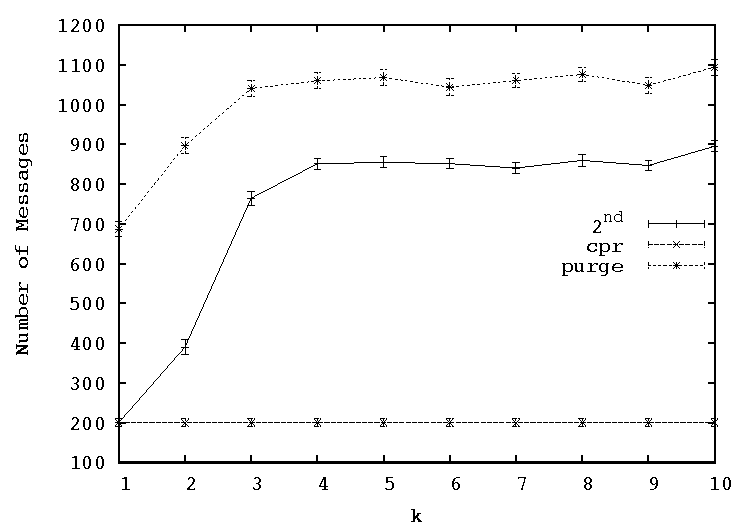
\includegraphics[scale=0.47]{figs/synch/msg5.pdf}}
%\subfigure[{Experiment 2 and 4}]{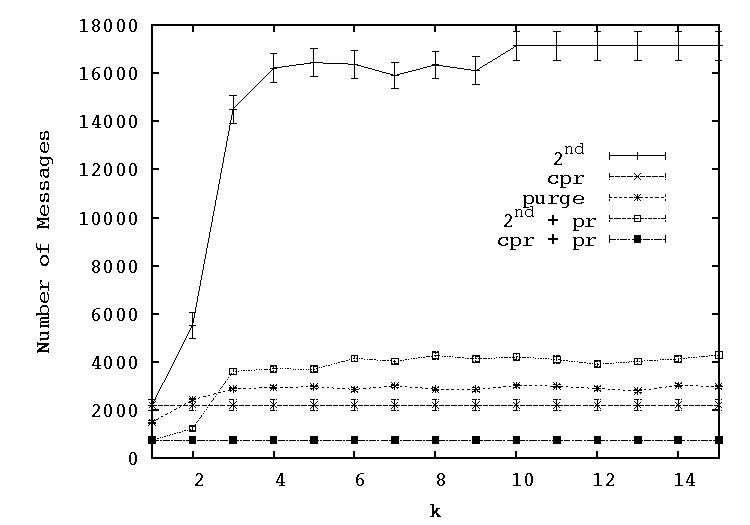
\includegraphics[scale=0.48]{figs/synch/msg-rand-pr5.pdf}}
%\subfigure[{Experiment 1}]{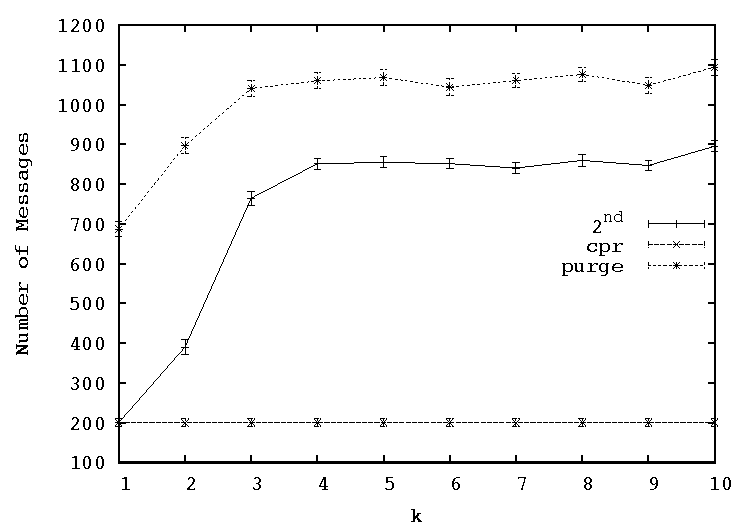
\includegraphics[width=0.49\textwidth]{figs/synch/msg5.pdf}}
\subfigure[{Single Compromised Node}]{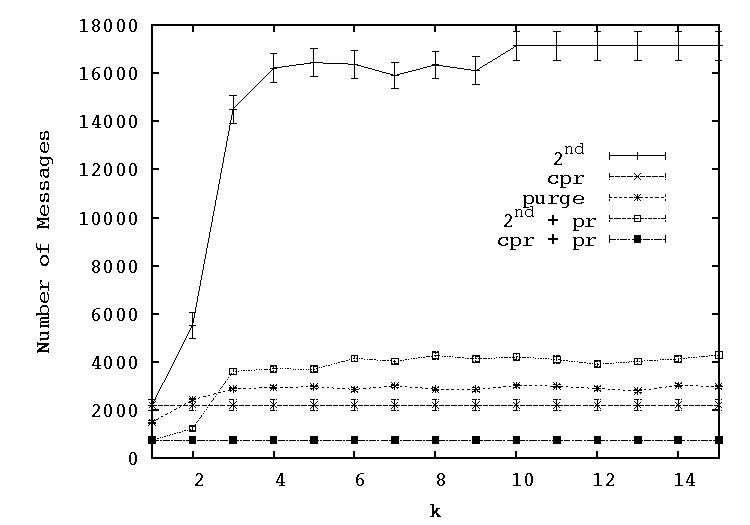
\includegraphics[width=0.32\textwidth]{figs/synch/msg-rand-pr5.pdf}}
\subfigure[{Multiple Compromised nodes}]{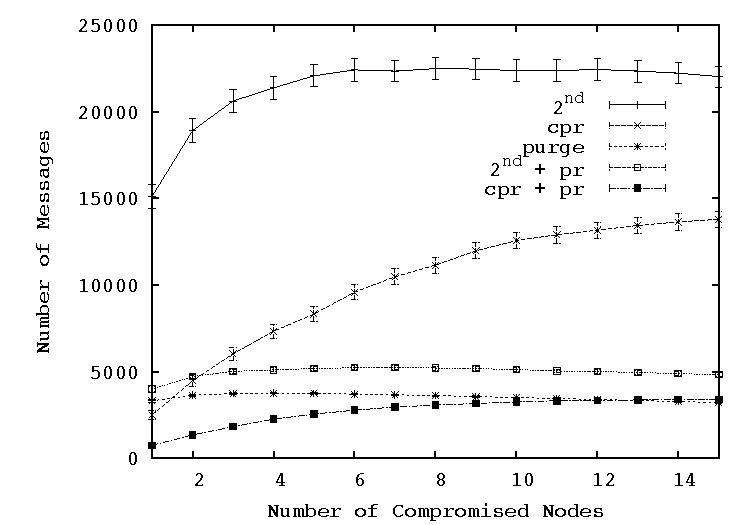
\includegraphics[width=0.32\textwidth]{figs/synch/many-pr-rand5.pdf}}
\caption{Experiment 5 plots.  Algorithms run over \er graphs with random link weights, $n=100$, $p=.05$, and average diameter=$6.14$. 
\second + {\tt pr} refers to \second using poison reverse. Likewise, \cpr + {\tt pr} is \cpr using poison reverse.}
\label{fig:pr-fix}
\end{figure*}




\subsection{Link Weight Change Experiments}
\label{subsec:change}

So far, we have evaluated our algorithms over different topologies with fixed link costs in scenarios with single and multiple compromised nodes.
We found that \cpr using poison reverse outperforms the other algorithms because \cpr removes false
routing state with a single diffusing computation, rather than using an iterative distance vector process as in \second and \purges, and poison reverse removes
all pairwise routing loops that occur during \cpr recovery. 

In the next three experiments we evaluate our algorithms over graphs with changing link costs. We introduce link cost changes between the time \bad is compromised and when \bad is discovered 
(e.g., during $[t',t_b]$). 
In particular, let there be $\lambda$ link cost changes per timestep, where $\lambda$ is deterministic. 
To create a link cost change event, we choose a link (except for all $(v,\bar{v})$ links) whose link will change equiprobably among all links. 
The new link cost is selected uniformly at random from $[1,n]$. 

\subsubsection{Experiment 6 - Link Cost Changes}

Except for $\lambda$, our experimental setup is identical to the one in Experiment 2. We let $\lambda = \{1,4,8\}$. In order to isolate the effects of link costs changes,
we assume that \cpr checkpoints at each timestep.

Figure \ref{fig:lc} shows \purge yields the lowest message overhead for $p=.05$, but only slightly lower than \cprs. 
\cprs's message overhead increases with larger $k$ because there are more link cost change events to process. After \cpr rolls back, it must process all link cost
changes that occurred in $[t',t_b]$. 
In contrast, \second and \purge process some of the link cost change events during the interval $[t',t_b]$ as part of normal distance vector execution. 
In our experimental setup, these messages are not counted because 
they do not occur in Step 4 (i.e., as part of the recovery process) of our simulation scenario described in Section \ref{sec:eval}.

Our analysis further indicates that \second performance suffers because of the \infinity problem. %\purge and \second must 
The gap between \second and the other algorithms shrinks as $\lambda$ increases because as $\lambda$ increases, link cost changes have a larger effect on message overhead.


\begin{figure*}[t]
\centering
\subfigure[{$p=0.05$, diameter=$6.14, \lambda=1$}]{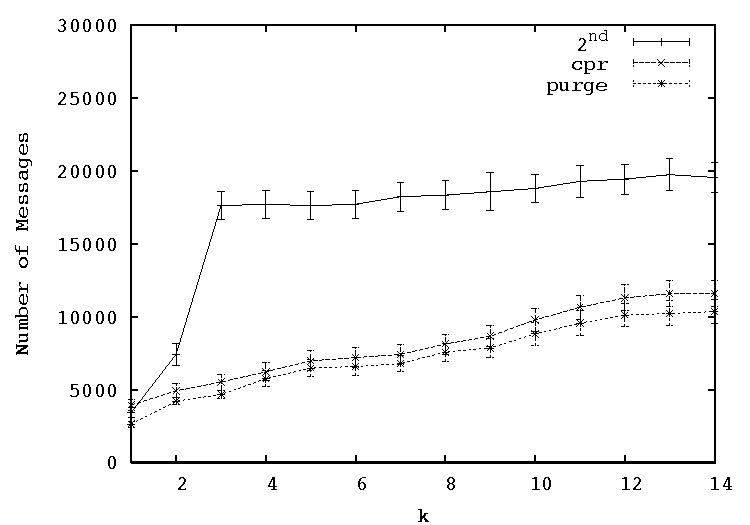
\includegraphics[width=0.32\textwidth]{figs/synch/p05-lc1.pdf}}
%\subfigure[{$p=0.05$, diameter=$6.14, \lambda=2$}]{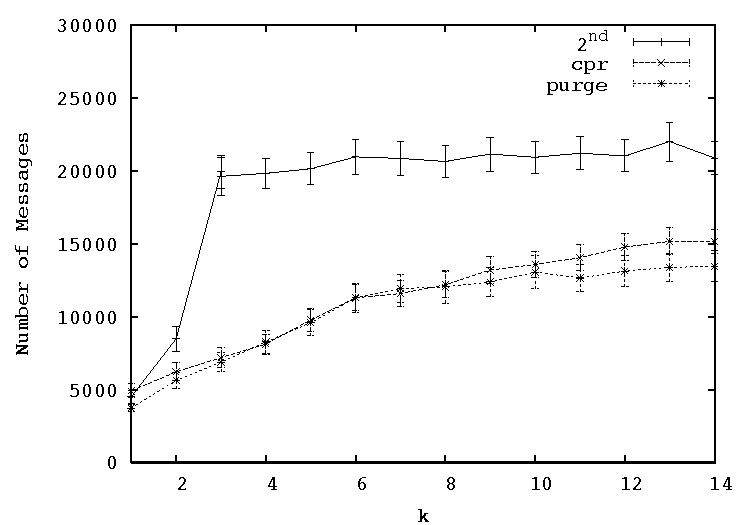
\includegraphics[width=0.32\textwidth]{figs/synch/p05-lc2.pdf}}
\subfigure[{$p=0.05$, diameter=$6.14,\lambda=4$}]{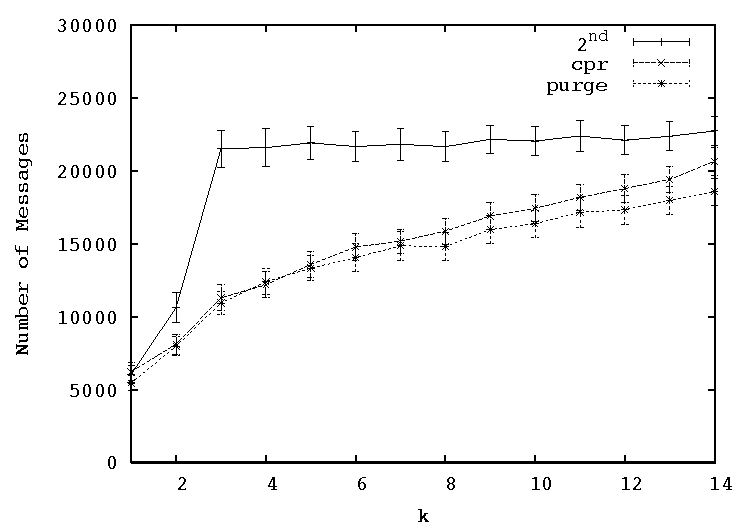
\includegraphics[width=0.32\textwidth]{figs/synch/p05-lc4.pdf}}
\subfigure[{$p=0.05$, diameter=$6.14, \lambda=8$}]{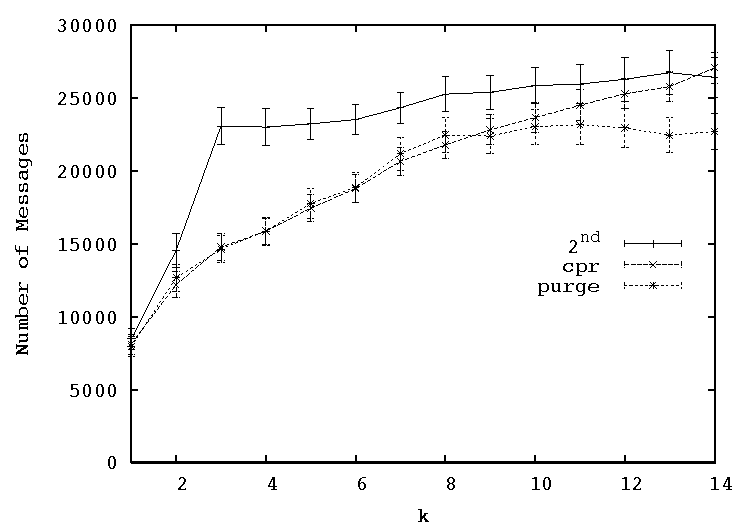
\includegraphics[width=0.32\textwidth]{figs/synch/p05-lc8.pdf}}
\subfigure[{$p=0.15$, diameter=$3.01, \lambda=1$}]{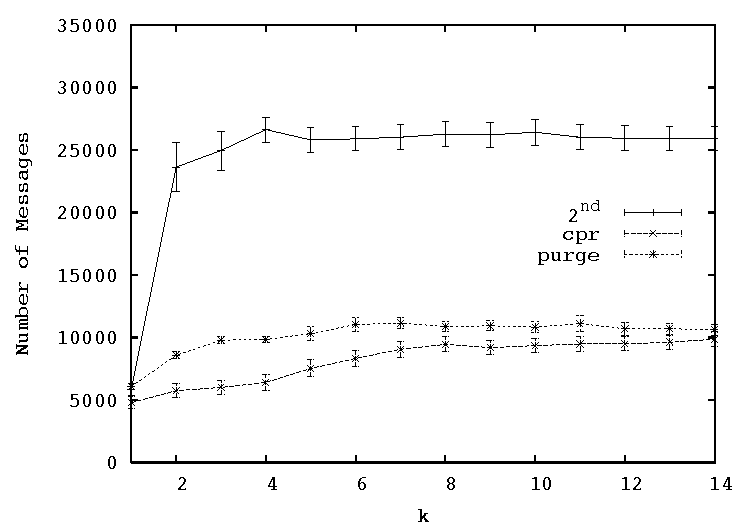
\includegraphics[width=0.32\textwidth]{figs/synch/p15-lc1.pdf}}
\subfigure[{$p=0.15$, diameter=$3.01,\lambda=4$}]{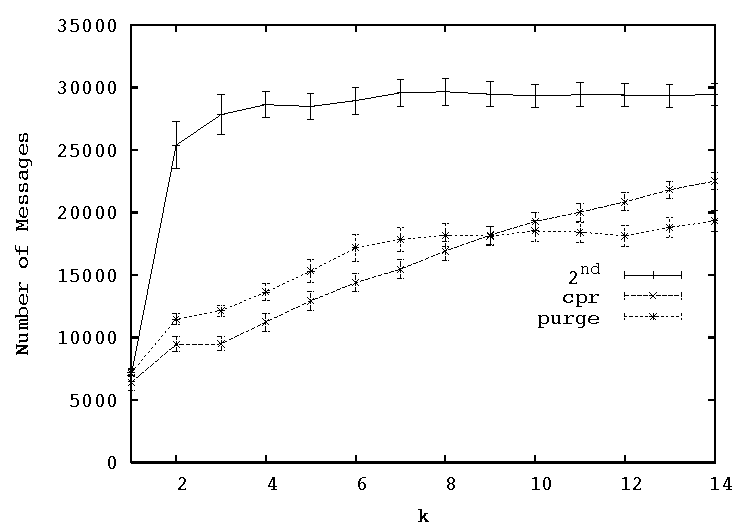
\includegraphics[width=0.32\textwidth]{figs/synch/p15-lc4.pdf}}
\subfigure[{$p=0.15$, diameter=$3.01, \lambda=8$}]{\includegraphics[width=0.32\textwidth]{figs/synch/p15-lc8.pdf}}
%\subfigure[{Cumulative path cost decreases during the simulation}]{\includegraphics[width=0.49\textwidth]{figs/tsdecrease6.pdf}}
\caption{Experiment 6: Message overhead for $p=\{0.05,0.15\}$ \er with link weights selected uniformly random with different $\lambda$ values.}
\label{fig:lc}
\end{figure*}

%\begin{figure*}[t]
%\centering
%\subfigure[{$p=0.15$, diameter=$3.01, \lambda=1$}]{\includegraphics[width=0.32\textwidth]{figs/synch/p15-lc1.pdf}}
%\subfigure[{$p=0.15$, diameter=$3.01,\lambda=4$}]{\includegraphics[width=0.32\textwidth]{figs/synch/p15-lc4.pdf}}
%\subfigure[{$p=0.15$, diameter=$3.01, \lambda=8$}]{\includegraphics[width=0.32\textwidth]{figs/synch/p15-lc8.pdf}}
%\subfigure[{Cumulative path cost decreases during the simulation}]{\includegraphics[width=0.49\textwidth]{figs/tsdecrease6.pdf}}
%\caption{Message overhead for $p=0.15$ \er with link weights selected uniformly random with different $\lambda$ values.}
%\label{fig:lc-p15}
%\end{figure*} 

With larger $p$ values, $\lambda$ has a smaller effect on message complexity because more alternate paths are available. Thus when $p=0.15$ and $\lambda=1$,
most of \purges's recovery effort is towards removing \badvector state, rather than processing link cost changes.  Because
\cpr removes \badvector using a single diffusing computation and there are few link cost changes, \cpr has lower message overhead than \purge in this case. 
As $\lambda$ increases, \cpr has higher message overhead than \purges: there are more link cost changes to process and \cpr must process all such link cost changes, 
while \purge processes some link cost changes during the interval $[t',t_b]$ as part of normal distance vector execution. 

\subsubsection{Experiment 7 - Poison Reverse and Link Cost Changes}
In this experiment, we apply poison reverse to each algorithm and repeat Experiment 6. Because \purges's diffusing computations only eliminate routing loops corresponding 
to \badvector state, \purge is vulnerable to routing loops stemming from link cost changes.  Thus, contrary to Experiment 5, poison reverse improves \purge performance.
The results are shown in Figure \ref{fig:prlc}. Each algorithm using poison reverse has label ``{\tt algorithm-name}'' + {\tt pr}).
Results for different $p$ values yield the same trends. 

All three algorithms using poison reverse show remarkable performance gains.
As confirmed by our profiling numbers, the improvements are significant because routing loops are more pervasive when link costs change.  
Accordingly, the poison reverse optimization yields greater benefits as $\lambda$ increases. % because larger $\lambda$ result in more routing loops. %for the standard \second and \cpr algorithms.

%Each algorithm using poison reverse is vulnerable to routing loops larger than $2$ that originate from link cost changes,
As in Experiment 5, we believe that for \badvector state \emph{only}, \purge + {\tt pr} removes routing loops larger than $2$ while \second + {\tt pr} does not. 
For this reason, we believe that \purge + {\tt pr} performs better than \second + {\tt pr}.  We are currently investigating this claim.
%As in Experiment 3, \second + {\tt pr} performs worse than \purge + {\tt pr} because we believe that for \badvector state \emph{only},
%\purge + {\tt pr} removes routing loops larger than $2$ while \second + {\tt pr} does not. Meanwhile, both 
% \second + {\tt pr} and \purge + {\tt pr} use poison reverse to address routing loops resulting from link cost changes.  Thus both algorithms (and \cpr + {\tt pr})
%are equally vulnerable to routing loops  larger than $2$ originating from link cost changes.
\cpr + {\tt pr} has the lowest message complexity. %among the three algorithms. 
In this experiment, the benefits of rolling back to a global snapshot taken before \bad was compromised outweigh the message overhead required to update stale state pertaining to 
link cost changes that occurred during $[t',t_b]$. As $\lambda$ increases,
the performance gap decreases because \cpr + {\tt pr} must process all link cost changes that occurred in $[t',t_b]$ while \second + {\tt pr}  and \purge + {\tt pr}
process some link cost change events during $[t',t_b]$ as part of normal distance vector execution.

%However, we make the strong performance of \cpr + {\tt pr} comes wiHh
However, \cpr + {\tt pr} only achieves such strong results by making two optimistic assumptions:  we assume perfectly synchronized clocks and checkpointing occurs at each timestep.
In the next experiment we relax the checkpointing assumption.
%However, we make two optimistic assumptions in order to achieve such favorable results for \cpr + {\tt pr}: we assume clocks are perfectly synchronized and checkpointing occurs at each timestep.
%In the next experiment we relax the checkpoint assumption.


\begin{figure*}[t]
\centering
\subfigure[{$p=0.05$, $\lambda=1$}]{\includegraphics[width=0.32\textwidth]{figs/synch/pr-p05-lc1.pdf}}
%\subfigure[{$p=0.05, \lambda=2$}]{\includegraphics[width=0.49\textwidth]{figs/synch/p05-lc2.pdf}}
\subfigure[{$p=0.05$, $\lambda=4$}]{\includegraphics[width=0.32\textwidth]{figs/synch/pr-p05-lc4.pdf}}
\subfigure[{$p=0.05$, $\lambda=8$}]{\includegraphics[width=0.32\textwidth]{figs/synch/pr-p05-lc8.pdf}}
%\subfigure[{Cumulative path cost decreases during the simulation}]{\includegraphics[width=0.49\textwidth]{figs/tsdecrease6.pdf}}
\caption{Plots for Experiment 7. Each figure shows message overhead for \er graphs with link weights selected uniformly at random, $p=0.05$, average diameter is $6.14$, and $\lambda=\{1,4,8\}$.
The curves for \second + {\tt pr}, \purge + {\tt pr}, and \cpr + {\tt pr} refer to each algorithm using poison reverse, respectively.
} 
\label{fig:prlc}
\end{figure*}


\subsubsection{Experiment 8 - Vary Checkpoint Frequency}

In this experiment we study the trade-off between message overhead and storage overhead for \cprs. To this end, we vary the frequency at which \cpr checkpoints and fix 
the interval $[t',t_b]$. Otherwise, our experimental setup is the same as Experiment 6.

Figure \ref{fig:lc-fixk} shows the results for an \er graph with link weights selected uniformly at random between $[1,n]$,
$n=100$, $p=.05$, $\lambda=\{1,4,8\}$ and $k=2$. We plot message overhead against the number of timesteps \cpr must rollback, $z$. \cprs's message overhead increases with larger $z$ 
because as $z$ increases there are more link cost change events to process. \second and \purge have constant message overhead because they operate independent of $z$.

We conclude that as the frequency of \cpr snapshots decreases, \cpr incurs higher message overhead.  Therefore, when choosing the frequency of checkpoints,
the trade-off between storage and message overhead must be carefully considered. 



\begin{figure*}[t]
\centering
\subfigure[{$p=0.05$, $k=2, \lambda=1$}]{\includegraphics[width=0.32\textwidth]{figs/synch/p05-k1.pdf}}
\subfigure[{$p=0.05$, $k=2, \lambda=4$}]{\includegraphics[width=0.32\textwidth]{figs/synch/p05-k4.pdf}}
\subfigure[{$p=0.05$, $k=2, \lambda=8$}]{\includegraphics[width=0.32\textwidth]{figs/synch/p05-k8.pdf}}
%\subfigure[{Cumulative path cost decreases during the simulation}]{\includegraphics[width=0.49\textwidth]{figs/tsdecrease6.pdf}}
\caption{Experiment 8: message overhead for $p=0.05$ \er with link weights selected uniformly random with different $\lambda$ values. $z$ refers to the number of timesteps \cpr must 
rollback. Note the y-axis have different scales.}
\label{fig:lc-fixk}
\end{figure*} 


\subsection{Summary}
\label{subsec:discuss}


Our results show \cpr using poison reverse yields the lowest message and time overhead in all scenarios. \cpr benefits from removing false state with a single
diffusing computation. Also, applying poison reverse significantly reduces \cpr message complexity by eliminating pairwise routing loops resulting from
link cost changes. However, \cpr has storage overhead, requires loosely synchronized clocks, and requires the time \bad was compromised.

\seconds's performance is determined by the \infinity problem. In the case of \er graphs with fixed unit link weights, the \infinity problem was minimal, 
helping \second perform better than \purges. % In all other scenarios, poison reverse significantly improves \second performance because routing loops are pervasive.
For all other topologies, poison reverse significantly improves \second performance because routing loops are pervasive.
Still, \second using poison reverse is not as efficient as \cpr and \purge using poison reverse.

In cases where link costs change, we found that \purge using poison reverse is only slightly worse than \cpr + {\tt pr}. % with poison reverse. 
Unlike \cprs, \purge makes use of computations that follow the injection of false state, that do not depend on false routing state.  
Because \purge does not make the assumptions that \cpr requires, \purge using poison reverse is a suitable alternative for topologies with link cost changes.
%In contrast to \cprs, \purge makes no assumptions 
%other than the identification of \bads, making \purge a suitable algorithm for topologies with link cost changes.

%\purge avoids the \infinity problem by first globally invalidating false state.  Therefore in cases where the \infinity problem is 
%significant, \purge outperforms \seconds.

%When considering graphs with changing link costs, \cprs's performance suffers because it must process all valid link cost changes that occurred since \bad was compromised.
%Meanwhile, \second and \purge make use of computations that followed the injection of false state, that do not depend on false routing state. However, \seconds's performance degrades 
%because of the \infinity problem.  \purge eliminates the \infinity problem and therefore yields the best performance over topologies with changing link costs.

Finally, we found that an additional challenge with \cpr is setting the parameter which determines checkpoint frequency.
Frequent checkpointing yields lower message and time overhead at the cost of more storage overhead. Ultimately, application-specific factors must be considered
when setting this parameter. 


\section{Related Work}
\label{sec:related-pmu}

\full is well-studied \cite{Baldwin93,Brueni05,Haynes02, Mili90, Xu04}.  
Haynes et al. \cite{Haynes02} and Brueni and Heath \cite{Brueni05} both prove \full is NPC.  
However, their proofs make the unrealistic assumption that all nodes are zero-injection.  We drop this assumption and thereby generalize their NPC results for \fulls.
Additionally, we leverage the proof technique from Brueni and Heath \cite{Brueni05} in all four of our NPC proofs, although our proofs
differ considerably in their details. 

%The power systems literature generally ignores the fact that PMUP is NP-Complete because, in practice, power system graphs are small enough to allow for an exact solution to be found.
In the power systems literature, Xu and Abur \cite{Xu04,Xu05} use integer programming to solve \fulls, while Baldwin et al. \cite{Baldwin93} and Mili et al. \cite{Mili90} use simulated annealing 
to solve the same problem. All of these works allow nodes to be either zero-injection or non-zero-injection.  However,
these papers make no mention that \full is NPC, i.e., they do not characterize the fundamental complexity of the problem. 
%The work of Xu and Abur \cite{Xu04} and Phadke et al. are representive of the power systems approach to the problem: formulate the problem as integer 
%program and use an integer programming solver to find the optimal PMU placement.  

Aazami and Stilp \cite{Aazami07} investigate approximation algorithms for \fulls.  They derive a hardness approximation threshold of $2^{\log^{1 -\epsilon}n}$.
Also they prove that in the worst case, {\tt greedy} from Section \ref{sec:approx} does no better $\Theta(n)$ of the optimal solution.  However, this approximation ratio assumes that 
all nodes are zero-injection.
%We leverage this approximation result in proving the approximation ratios of our heuristic-based algorithms.

Chen and Abur \cite{Abur06} and Vanfretti et al. \cite{Vanfretti10} both study the problem of bad PMU data. Chen and Abur \cite{Abur06} formulate their problem differently than \xval and \xvalparts.  
They consider fully observed graphs and add PMUs to the system to make all existing PMU measurements non-critical 
(a critical measurement is one in which the removal of a PMU makes the system
no longer fully observable). Vanfretti et al. \cite{Vanfretti10} define the cross-validation rules used in this paper.  They also derive a
lower bound on the number of PMUs needed to ensure all PMUs are cross-validated and the system is fully observable. 



\section{Conclusions and Future Work}
\label{sec:future}

In this paper, we developed methods for recovery in scenarios where a malicious node injects false state into a distributed system.  
We studied an instance of this problem in distance vector routing.
We presented and evaluated three new algorithms for recovery in such scenarios. %from false state in distance vector routing 
Among our three algorithms, our results show that \cpr -- a checkpoint-rollback based algorithm -- yields the lowest message and time overhead over topologies
with fixed link costs.  However, \cpr has storage overhead and requires loosely synchronized clocks.
In the case of topologies with changing link costs, \purge performs best by avoiding the problems that plague \cpr and \seconds.
Unlike \cprs, \purge has no stale state to update because \purge does not rollback in time.  
The \infinity problem results in high message overhead for \seconds, while \purge eliminates the \infinity problem by globally purging false state before finding new least cost paths.

As future work, we are interested in finding the worst possible false state a compromised node can inject.  Some options include the minimum distance to all nodes (e.g., 
our choice for false state used in this paper), state that maximizes the effect of the \infinity problem, and false state that contaminates a bottleneck link. 
We also would like to evaluate the effects of multiple compromised nodes on our recovery algorithms. 



\section{Acknowledgments}
The authors greatly appreciate discussions with Dr. Brian DeCleene of BAE Systems, who initially suggested this problem area.


\bibliographystyle{plain}
\bibliography{infocom}

%%%%%%%%%%% Appendix %%%%%%%%%%%%%%%%%%
\section{Appendix}
\label{sec:appendix}

%%%%%%%%%%%%%%% 2nd Best ALG PART 1 %%%%%%%%%%%%%%%%%%%%%%%%%%%%%%
\begin{algorithm}
\caption{\seconds}
\label{alg:second}
%\textsc{centralized-dv}($G$)

\begin{algorithmic}[1]
%\STATE{$t_i \leftarrow t_0$}

\STATE{$flag \leftarrow$ \textsc{false}}
\STATE{set distance to \bad to $\infty$ in \minvi and \dmatrixi}
\FOR{{\bf each} destination $d$ }
	\IF{route via \bad to reach $d$}
		\STATE{select new shortest distance to $d$ which does not route via \bads. Update \minvi and \dmatrixi with this value.}
		\STATE{$flag \leftarrow$ \textsc{true}} 
	\ENDIF
\ENDFOR
	\IF{$flag$ $=$ \textsc{true}}
		\STATE{send \minvi to each  $j \in adj(i)$ where $j \neq$ \bads }
	\ENDIF

\end{algorithmic}
\end{algorithm}




%%%%%%%%%%%%%%% Purge's Purge Phase ALG PART 1 %%%%%%%%%%%%%%%%%%%%%%%%%%%%%%
\begin{algorithm}
\caption{\purges's purge phase}
\label{alg:purge}
%\textsc{centralized-dv}($G$)

\begin{algorithmic}[1]
\STATE{set distance to \bad to $\infty$}
\FOR{{\bf each} destination $d$}
	\IF{route via \bad to reach $d$}
		\STATE{$S \leftarrow S \cup \{d\}$} 
	\ENDIF
\ENDFOR
	
\IF{$S$ is not empty}
	\STATE{send $S$ to each $j \in adj(i)$ where $j \neq$ \bads }
\ENDIF

\end{algorithmic}
\end{algorithm}


%%%%%%%%%%%%%%% Purge's Purge Phase ALG PART 2 %%%%%%%%%%%%%%%%%%%%%%%%%%%%%%
\begin{algorithm}
\caption{\purges's purge phase}
\label{alg:purge2}
%\textsc{centralized-dv}($G$)

\begin{algorithmic}[1]

\FOR{{\bf each} $d \in msg.dests$}
	\IF{route via message source to $d$}
		\STATE{$S \leftarrow S \cup \{d\}$} 
	\ENDIF
\ENDFOR
\IF{$S$ is not empty}
	\STATE{send $S$ to each $j \in adj(i)$ where $j \neq$ \bads }
\ELSE
	\STATE{send $ACK$ to message source}
\ENDIF

\end{algorithmic}
\end{algorithm}



%%%%%%%%%%%%%%% Purge's Discover Phase ALG PART 1%%%%%%%%%%%%%%%%%%%%%%%%%%%%%%
\begin{algorithm}
\caption{\purges's discovery phase}
\label{alg:discover}

\begin{algorithmic}[1]
\STATE{$flag \leftarrow$ \textsc{false}}
\FOR{{\bf each} destination $d$}
	\IF{\minvis$[d] = \infty$}
		\STATE{find shortest distance in \dmatrixi and set in \minvis}
		\STATE{$flag \leftarrow$ \textsc{true}} 
	\ENDIF
\ENDFOR
\IF{$flag$ $=$ \textsc{true}}
	\STATE{send \minvi to each  $j \in adj(i)$ where $j \neq$ \bads }
\ENDIF


\end{algorithmic}
\end{algorithm}

%%%%%%%%%%%%%%% Purge's Discover Phase ALG PART 2 %%%%%%%%%%%%%%%%%%%%%%%%%%%%%%
\begin{algorithm}
\caption{\purges's discovery phase}
\label{alg:discover2}

\begin{algorithmic}[1]
\IF{first round of sending}
	\FOR{{\bf each} destination $d$}
		\STATE{update \minvi with minumum distance in \dmatrixi to $d$}
	\ENDFOR
\ENDIF
\STATE{run distance vector} 

\end{algorithmic}
\end{algorithm}


%%%%%%%%%%%%%%% CPR ALG PART 1 %%%%%%%%%%%%%%%%%%%%%%%%%%%%%%
\begin{algorithm}
\caption{\cpr steps after rollback}
\label{alg:cpr}

\begin{algorithmic}[1]

\STATE{$flag \leftarrow$ \textsc{false}}
\FOR{{\bf each} destination $d$}
	\IF{\minvis$[d] = \infty$}
		\STATE{find shortest distance in \dmatrixi and set in \minvis}
		\STATE{$flag \leftarrow$ \textsc{true}} 
	\ENDIF
\ENDFOR
\IF{$flag$ $=$ \textsc{true} or adjacent link weight changed during $[t',t]$}
	\STATE{send \minvi to each  $j \in adj(i)$ where $j \neq$ \bads }
\ENDIF



\end{algorithmic}
\end{algorithm}


%%%%%%%%%%%%%%% CPR ALG PART 2 %%%%%%%%%%%%%%%%%%%%%%%%%%%%%%
\begin{comment}
\begin{algorithm}
\caption{\cpr steps after rollback}
\label{alg:cpr}

\begin{algorithmic}[1]
	\IF{first round of sending}
		\STATE{update \minvi with most recent link weights of adjacent link}
	\ENDIF
	\STATE{run distance vector} 
\ENDIF


\end{algorithmic}
\end{algorithm}

\end{comment}







%\section{Todo}

{\bf Writing Todos}

{\it 
\begin{itemize}

	\item do all of our recovery algorithms requires loose synchronization assumption since the oracle notification includes time $t'$?

	\item if there is a \lcd then the node must send

\end{itemize}
}

{\bf Miscallaneous Text}

\begin{itemize}
	\item Although we only explicitly consider flat topologies, we believe that the recovery algorithms studied in this work can be applied to hierarchical topologies. 
	{\it this text was in the Problem Formulation section, at the end of the first paragraph}

\end{itemize}




\end{document}
